% Sesión 9: integración de S09a, S09b y S09c.
\section{Dónde quedamos}

\begin{obs}[Fe de erratas de la 8d]
\label{obs:s09-erratas-ocho}
\begin{enumerate}
\item \emph{Primitivo.} Los primos no nulos de $\mathbb Z[t]$ sobre $(0)$ son los $(g)$ con $g$ no constante, primitivo e irreducible. Primitivo significa que el máximo común divisor de sus coeficientes, el contenido, es $1$. El polinomio $2t-1$ es primitivo y no es mónico.
\item \emph{El cociente de $(p,g)$.} Si $\bar g$ es la reducción de $g$ módulo $p$, entonces $\mathbb Z[t]/(p,g)\cong\mathbb F_p[t]/(\bar g)$.
\item \emph{Los no máximos.} Los ideales $(0)$, $(p)$ y $(g)$ son primos y no son máximos. El ideal $(p,g)$, con $\bar g$ irreducible en $\mathbb F_p[t]$, es máximo y contiene estrictamente a $(p)$ y a $(g)$; véase la \cref{prop:s08-primos-z-t}.
\item \emph{Sobre el primo $2$.} La curva $V(t^2+1)$ tiene un solo punto doble sobre $(2)$, pues $t^2+1=(t+1)^2$ en $\mathbb F_2[t]$.
\item \emph{Sobre $3$ y $7$.} Hay un solo punto, de grado $2$. Hay dos puntos de grado $1$ si y solo si $p\equiv1\pmod4$, como sobre $5$. El grado de un punto cerrado es $[\kappa(x):\mathbb F_p]$; véanse la \cref{prop:s08-puntos-curva-gaussiana} y Vakil, \S5.3.8.
\item \emph{El disco.} El dibujo del disco con su centro representa $\Spec\mathbb Z_{(p)}$, la localización de $\mathbb Z$ en $(p)$. El disco topológico sin el centro tiene grupo fundamental $\mathbb Z$.
\item \emph{Fibra genérica y fibra especial.} La fibra sobre $(0)$ es la genérica y la fibra sobre el ideal máximo $(p)$ de $\mathbb Z_{(p)}$ es la especial. La reducción de un punto racional de la fibra genérica es un punto de la fibra especial.
\item \emph{Símbolo de Legendre.} El símbolo $\left(\frac ap\right)$ vale $1$ si $a$ es un cuadrado no nulo módulo $p$, $-1$ si no es un cuadrado y $0$ si $p\mid a$. Para $p$ impar, $-1$ es un cuadrado módulo $p$ si y solo si $p\equiv1\pmod4$.
\item \emph{Lema de Gauss.} Para $g\in\mathbb Z[t]$ primitivo, $g\mathbb Q[t]\cap\mathbb Z[t]=g\mathbb Z[t]$; véanse la \cref{prop:s08-gauss} y Lang, \emph{Algebra}, cap.~IV, \S2.
\end{enumerate}
\end{obs}

La clase anterior calculó los primos de $\mathbb Z[t]$, dibujó el mapa de Mumford de $\Spec\mathbb Z[t]$ con $V(t^2+1)$, vio $\mathbb P^1_{\mathbb Z}$ como superficie aritmética y presentó el espectro de un DVR como un disco con su centro. Retomamos la reducción de puntos racionales para explicarla con sus ecuaciones.

\begin{obs}[Qué buscamos hoy]
\label{obs:s09-objetivos}
\begin{enumerate}
\item \emph{Valoración discreta.} La valuación $v$ de un DVR y el disco con su centro.
\item \emph{Reducción y buena reducción.} Reducir un punto de $\mathbb P^1_K$ y su ecuación; definir cuándo un esquema sobre $K$ tiene buena reducción, con $\Spec\mathbb Z[i]\to\Spec\mathbb Z$ como modelo guía.
\item \emph{Primos sobre $(0)$ y sobre $\mathfrak m$.} Describir los primos de $A[x]/(f)$ mediante $K[x]/(f)$ y $\kappa[x]/(\bar f)$.
\item \emph{$\mathbb P^n_A$.} Las cartas y los morfismos de pegado, sin repetir el desarrollo de $\mathbb P^1_A$.
\item \emph{Propiedades básicas.} Reducido, irreducible, integral y noetheriano, con $\Spec k[\varepsilon]/(\varepsilon^2)$ y $\Spec k[x,y]/(xy)$. La fibra no reducida de $\Spec\mathbb Z[i]$ sobre $2$ motiva la primera.
\end{enumerate}
La definición de modelo queda aplazada con el alcance de la \cref{obs:s09-lo-que-se-aplaza}.
\end{obs}

\begin{obs}[Quedan de ejercicio]
\label{obs:s09-ejercicios-repaso}
Queda como ejercicio demostrar que $(p,g)$ no es principal y que un primo de $\mathbb Z[t]$ es máximo si y solo si no es principal, así como estudiar los puntos de $\mathbb P^1$ sobre cuerpos finitos con su conteo por la función de Möbius, y el ejemplo $(6,t)$. Las secciones $t=0$ y $t=2$ con el punto $(2,t)$ se retoman en el \cref{ejem:s09-misma-reduccion}, y el isomorfismo $\mathbb Z[t]/(t^2+1)\cong\mathbb Z[i]$ en el \cref{ejem:s09-enteros-gaussianos}.
\end{obs}

\section{Lo que se usa hoy}
Todo anillo es conmutativo y con unidad. Las referencias a Vakil son a \emph{The Rising Sea}: los materiales de valoración y reducción siguen el borrador del 8 de septiembre de 2024, y el de propiedades básicas indica el del 21 de octubre de 2025. Las referencias a Liu son a \emph{Algebraic Geometry and Arithmetic Curves}. Recordamos aquí las herramientas para los argumentos siguientes.

\subsection{Espectro, puntos y pegado}

\begin{defi}[Espectro, abiertos básicos y cerrados]
\label{defi:s09-espectro}
El espectro $\Spec A$ es el conjunto de ideales primos de $A$ con la topología de Zariski. Sus cerrados son $V(I)=\set{\mathfrak p\in\Spec A\given I\subseteq\mathfrak p}$ y los $D(f)=\set{\mathfrak p\in\Spec A\given f\notin\mathfrak p}$ forman una base de abiertos. Su gavilla estructural cumple $\mathcal O(D(f))=A_f$, $D(f)\cong\Spec A_f$ y $\mathcal O_{\Spec A,\mathfrak p}=A_{\mathfrak p}$. Se tiene $V(I)=V(\sqrt I)$ porque un primo contiene a $I$ si y solo si contiene a $\sqrt I$; también $V(ab)=V(a)\cup V(b)$, por primalidad, y $V(I)\cap V(J)=V(I+J)$. \emph{[Sesiones 1, 2 y 5.]}
\end{defi}

\begin{defi}[Puntos cerrados, genéricos y especializaciones]
\label{defi:s09-especializaciones}
Un punto $x$ es cerrado si $\set{x}$ es cerrado, es genérico de un cerrado $Z$ si $Z=\overline{\set{x}}$, y $y$ es una especialización de $x$ si $y\in\overline{\set{x}}$. En $\Spec A$, un punto es cerrado si y solo si su ideal es máximo, y $\overline{\set{\mathfrak p}}=V(\mathfrak p)$. Si $A$ es un dominio, $(0)$ es el genérico. \emph{[Sesión 2; Vakil, \S3.6.]}
\end{defi}

\begin{defi}[Cuerpo residual]
\label{defi:s09-cuerpo-residual}
Para $\mathfrak p\in\Spec A$, $\kappa(\mathfrak p)=A_{\mathfrak p}/\mathfrak pA_{\mathfrak p}=\Frac(A/\mathfrak p)$. Si $A$ es local con ideal máximo $\mathfrak m$, entonces $\kappa(\mathfrak m)=A/\mathfrak m$. En un esquema, $\kappa(x)=\mathcal O_{X,x}/\mathfrak m_x$, con $\mathfrak m_x$ el máximo del anillo local $\mathcal O_{X,x}$. \emph{[Sesiones 1 y 5.]}
\end{defi}

\begin{prop}[Anillos locales y dominios de ideales principales]
\label{prop:s09-locales-dip}
\begin{enumerate}[label=(\alph*)]
\item En un anillo local $A$, un elemento es unidad si y solo si no está en su ideal máximo $\mathfrak m$; este es el conjunto de las no unidades.
\item En un dominio de ideales principales todo primo no nulo es máximo.
\item Toda localización de un dominio de ideales principales en un conjunto multiplicativo sin el $0$ es otro dominio de ideales principales.
\item En un dominio de ideales principales, la unión de una cadena ascendente de ideales es principal y su generador está en un eslabón. Por ello toda cadena ascendente se estaciona.
\end{enumerate}
\emph{[Atiyah--Macdonald, cor.~1.5 y cap.~3; Dummit--Foote, \S8.2.]}
\end{prop}

\begin{prop}[Polinomios sobre un cuerpo]
\label{prop:s09-polinomios-cuerpo}
Si $f\in k[t]$ es irreducible de grado $d$, con $k$ un cuerpo, entonces $k[t]/(f)$ es un cuerpo con $k$-base $1,t,\ldots,t^{d-1}$; si $k=\mathbb F_p$, tiene $p^d$ elementos. Para $a\ne b$, los ideales $(t-a)$ y $(t-b)$ son comaximales, y el teorema chino de la \cref{prop:s09-productos-chino} da $k[t]/((t-a)(t-b))\cong k\times k$. \emph{[Lang, \emph{Algebra}, cap.~IV, \S1; \cref{prop:s08-polinomios-campo}.]}
\end{prop}

\begin{prop}[La ecuación $x^2=-1$ módulo $p$]
\label{prop:s09-menos-uno-cuadrado}
Sea $p$ un primo impar. El elemento $-1$ es un cuadrado en $\mathbb F_p$ si y solo si $p\equiv1\pmod4$. \emph{[Lang, \emph{Algebra}, cap.~IV, \S1, para la ciclicidad de $\mathbb F_p^\times$.]}
\end{prop}
\begin{proof}
Si $a^2=-1$, entonces $a$ tiene orden $4$ en $\mathbb F_p^\times$, pues $-1\ne1$. Por Lagrange, $4\mid(p-1)$. Recíprocamente, si $4\mid(p-1)$ y $g$ genera el grupo cíclico $\mathbb F_p^\times$, el elemento $a=g^{(p-1)/4}$ tiene orden $4$. Su cuadrado es el único elemento de orden $2$, que es $-1$. La ciclicidad se recordó en la \cref{prop:s08-cuerpos-finitos}.
\end{proof}

\begin{defi}[Datos de pegado y Lema de Pegado]
\label{defi:s09-datos-pegado}
Los datos de pegado para $\set{X_i}_{i\in I}$ son abiertos $X_{ij}\subseteq X_i$, con $X_{ii}=X_i$, e isomorfismos $\varphi_{ij}:X_{ij}\to X_{ji}$ tales que (P1) $\varphi_{ii}=\id$, (P2) $\varphi_{ji}=\varphi_{ij}^{-1}$ y (P3) $\varphi_{ij}(X_{ij}\cap X_{ik})=X_{ji}\cap X_{jk}$ y $\varphi_{ik}=\varphi_{jk}\circ\varphi_{ij}$ en $X_{ij}\cap X_{ik}$. El \myref{teo:s07-lema-pegado} produce $X$ e inmersiones abiertas $\psi_i:X_i\to X$ cuyas imágenes lo cubren, con $\psi_i(X_i)\cap\psi_j(X_j)=\psi_i(X_{ij})$ y $\psi_j\circ\varphi_{ij}=\psi_i$ en $X_{ij}$, únicos salvo un único isomorfismo compatible. \emph{[Vakil, \S4.4.4 y ej.~4.4.A; Hartshorne, II.2, ej.~2.12.]}
\end{defi}

\subsection{Para la valoración discreta y la reducción}

\begin{defi}[La recta proyectiva $\mathbb P^1_A$ y sus puntos]
\label{defi:s09-recta-proyectiva}
La recta proyectiva se obtiene pegando $U_0=\Spec A[t]$ y $U_1=\Spec A[s]$ mediante $A[s,s^{-1}]\to A[t,t^{-1}]$, $s\mapsto t^{-1}$, sobre $D(s)$ y $D(t)$. Lleva el morfismo estructural $\pi:\mathbb P^1_A\to\Spec A$. Sobre un cuerpo $k$ sus puntos son $(0)$, los $(f)$ con $f$ mónico irreducible, e $\infty=(s)$; las fibras sobre $\mathfrak p$ tienen los puntos de $\mathbb P^1_{\kappa(\mathfrak p)}$. Para un cuerpo $F$, $\mathbb P^1(F)$ denota las clases $[a:b]$ de pares de $F^2\setminus\set{(0,0)}$ módulo $F^\times$. Se identifican con los puntos de grado $1$ por $[a:b]\mapsto(t-b/a)$ si $a\ne0$ y $[0:1]\mapsto\infty$. \emph{[Sesión 8; Vakil, \S4.4.6 y \S4.4.9.]}
\end{defi}

\begin{defi}[Formas binarias y sus ceros]
\label{defi:s09-formas-binarias}
Una forma binaria de grado $d$ sobre un cuerpo $F$ es un polinomio homogéneo $f=\sum_{i=0}^d c_iX^{d-i}Y^i\in F[X,Y]$. Un cero en $\mathbb P^1(F)$ es una clase $[a:b]$ con $f(a,b)=0$; no depende del representante porque $f(\lambda a,\lambda b)=\lambda^df(a,b)$. \emph{[Liu, \S10.1.1, ej.~1.4.]}
\end{defi}

\subsection{Para las propiedades básicas}
\subsubsection{Definiciones}

\begin{defi}[Nilpotentes, anillos reducidos y radical]
\label{defi:s09-nilpotentes}
Un elemento $a$ es nilpotente si $a^n=0$ para algún $n\ge1$. Los nilpotentes forman el nilradical $\Nil(A)$. El anillo $A$ es reducido si $\Nil(A)=0$; el anillo cero es reducido. Un dominio es un anillo no nulo sin divisores de cero, y es reducido: si $a^n=0$ con $n$ mínimo y $n\ge2$, de $a\,a^{n-1}=0$ se obtiene $a=0$ o $a^{n-1}=0$, contradiciendo esa elección. El radical de $I$ es $\sqrt I=\set{a\in A\given a^n\in I\text{ para algún }n\ge1}$, y $\sqrt I/I=\Nil(A/I)$. \emph{[Vakil, \S3.2.12--3.2.14 y ej.~3.2.R; Atiyah--Macdonald, cap.~1.]}
\end{defi}

\begin{obs}[La especialización es local]
\label{obs:s09-especializacion-local}
Si $y\in\overline{\set{x}}$ y un abierto $U$ contiene a $y$, entonces $x\in U$: toda vecindad de $y$ corta a $\set{x}$. Si $S\subseteq Y\subseteq X$, su cerradura en $Y$ es $\overline S^{\,X}\cap Y$. \emph{[\Cref{obs:s08-especializacion-local}; Vakil, ej.~3.6.N.]}
\end{obs}

\begin{defi}[Germen, tallo y valor]
\label{defi:s09-germen-tallo-valor}
Para $s\in\mathcal O_X(U)$ y $x\in U$, el germen $s_x$ es su clase en $\mathcal O_{X,x}$. Todo elemento del tallo es un germen; dos secciones tienen el mismo germen si coinciden en un entorno de $x$. El tallo es local, con ideal máximo $\mathfrak m_x$ formado por las no unidades. El valor $s(x)\in\kappa(x)$ es la clase de $s_x$; se anula si $s_x\in\mathfrak m_x$. Si $x\in V\subseteq U$ con $V$ abierto, $(s|_V)_x=s_x$ y $\mathcal O_{X,x}=\mathcal O_{V,x}$. \emph{[Vakil, \S2.2.3--2.2.5, \S4.3.6--4.3.7 y ej.~2.4.A; Sesión 5.]}
\end{defi}

\begin{prop}[Tallos y valores en $\Spec A$]
\label{prop:s09-tallos-valores-afin}
En $\mathfrak p\in\Spec A$ el tallo es $A_{\mathfrak p}$, con ideal máximo $\mathfrak pA_{\mathfrak p}$ y cuerpo residual $\kappa(\mathfrak p)$. El germen de $a\in A$ es $a/1$, y $a/1\in\mathfrak pA_{\mathfrak p}$ si y solo si $a\in\mathfrak p$. Por tanto $a(\mathfrak p)=0$ si y solo si $a\in\mathfrak p$, y su germen es unidad si y solo si $a\notin\mathfrak p$. \emph{[Vakil, ej.~4.1.E; Atiyah--Macdonald, prop.~3.11(iv).]}
\end{prop}

\begin{defi}[Abiertos afines, uniones disjuntas y cartas de $\mathbb P^n_A$]
\label{defi:s09-afines-disjuntas-cartas}
Un esquema es un espacio localmente anillado cubierto por abiertos isomorfos a espectros afines. Los abiertos afines contenidos en un abierto $U$ cubren $U$: si $x\in U\cap\Spec A$, los básicos $D(f)\cong\Spec A_f$ contenidos en esa intersección son una base.

Para una familia $\set{X_i}_{i\in I}$, los datos con $X_{ii}=X_i$ y $X_{ij}=\varnothing$ si $i\ne j$ cumplen (P1)--(P3). Su pegado es $\coprod_i X_i$; las imágenes de las inmersiones $\psi_i$ son abiertas, cubren el esquema y son disjuntas, pues $\psi_i(X_i)\cap\psi_j(X_j)=\psi_i(X_{ij})=\varnothing$.

El esquema $\mathbb P^n_A$ de la \cref{defi:s09-cartas-proyectivas} es la unión $\bigcup_i\psi_i(U_i)$ de $n+1$ cartas $U_i=\Spec A_i$, con $A_i$ un anillo de polinomios en $n$ variables sobre $A$. \emph{[Sesiones 7 y 8; Vakil, \S4.4.9--4.4.10.]}
\end{defi}

\begin{defi}[Espacios conexos, cuasicompactos y noetherianos]
\label{defi:s09-topologia-finita}
Un espacio es conexo si no es unión de dos abiertos disjuntos no vacíos. Una componente conexa es un subconjunto conexo maximal; las componentes son disjuntas y cubren el espacio. Dos subconjuntos conexos con un punto común tienen unión conexa. Un espacio es cuasicompacto si todo cubrimiento abierto admite un subcubrimiento finito, y es noetheriano si toda cadena descendente de cerrados se estabiliza. Todo $\Spec A$ es cuasicompacto y toda unión finita de subespacios cuasicompactos es cuasicompacta. \emph{[Vakil, \S3.6.2, \S3.6.5, \S3.6.14, ej.~3.6.G(a) y 3.6.H(a); topología general para las componentes conexas.]}
\end{defi}

\begin{defi}[Anillos noetherianos]
\label{defi:s09-anillos-noetherianos}
Un anillo es noetheriano si toda cadena ascendente de ideales se estabiliza; equivale a que todo ideal sea finitamente generado. Sus cocientes son noetherianos, por la correspondencia de ideales, y los dominios de ideales principales lo son por la \cref{prop:s09-locales-dip}(d). El teorema de la base de Hilbert afirma que $A[x_1,\ldots,x_n]$ es noetheriano si $A$ lo es. En particular, lo son $k[x_1,\ldots,x_n]$ y $\mathbb Z[x_1,\ldots,x_n]$. \emph{[Vakil, ej.~3.6.R, 3.6.S y \S3.6.16--3.6.19; Atiyah--Macdonald, caps.~6--7.]}
\end{defi}

\subsubsection{Hechos de álgebra}

\begin{prop}[Primos de un cociente]
\label{prop:s09-primos-cociente}
La aplicación $\mathfrak q\mapsto\mathfrak q/I$ es una biyección entre los primos de $A$ que contienen a $I$ y los de $A/I$, inversa a la contracción por $A\to A/I$. \emph{[Vakil, ej.~3.2.J; Atiyah--Macdonald, cap.~1; \cref{prop:s08-primos-cociente}.]}
\end{prop}

\begin{prop}[El nilradical es la intersección de los primos]
\label{prop:s09-nilradical}
Para todo anillo $A$ e ideal $I$,
\[
\Nil(A)=\bigcap_{\mathfrak p\in\Spec A}\mathfrak p,
\qquad \sqrt I=\bigcap_{\mathfrak p\supseteq I}\mathfrak p.
\]
En particular, $D(f)=\varnothing$ si y solo si $f$ es nilpotente. \emph{[Atiyah--Macdonald, prop.~1.8; Vakil, teo.~3.2.13; \cref{teo:s01-caracterizacion-nilradical}.]}
\end{prop}
La segunda igualdad es la primera aplicada a $A/I$, usando la \cref{prop:s09-primos-cociente}. La última afirmación expresa que $f$ está en todos los primos si y solo si es nilpotente.

\begin{prop}[Ideales máximos y primos minimales]
\label{prop:s09-maximos-minimales}
\begin{enumerate}[label=(\alph*)]
\item Todo ideal propio está contenido en un máximo, y todo máximo es primo. Por tanto, un ideal que no está contenido en ningún primo es todo el anillo.
\item Todo primo contiene un primo minimal, es decir, uno que no contiene propiamente a otro primo.
\end{enumerate}
\emph{[Atiyah--Macdonald, cap.~1 y ej.~1.8; Vakil, ej.~3.7.G.]}
\end{prop}
\begin{proof}
Para (a), los ideales propios que contienen a un ideal propio $I$ forman un conjunto no vacío. La unión de una cadena sigue siendo propia, pues si contuviera a $1$ algún eslabón lo contendría. Zorn da un máximo $\mathfrak m$. Si $ab\in\mathfrak m$ y $a\notin\mathfrak m$, escribimos $1=m+ra$ con $m\in\mathfrak m$; al multiplicar por $b$ resulta $b\in\mathfrak m$.

Para (b), ordenamos por inclusión inversa los primos contenidos en un primo fijo $\mathfrak p$. La intersección de una cadena es prima: si $ab$ está en todos sus miembros y $a$ no está en uno, digamos $\mathfrak q_0$, la primalidad da $b\in\mathfrak q_0$. En cualquier miembro mayor está $b$; en uno menor no está $a$, así que también está $b$. La intersección es propia, y Zorn produce un primo minimal dentro de $\mathfrak p$.
\end{proof}

\begin{prop}[Localización]
\label{prop:s09-localizacion}
En $S^{-1}A$ se tiene $a/s=b/t$ si y solo si $u(at-bs)=0$ para algún $u\in S$. En particular, $a/1=0$ si y solo si $ua=0$ para algún $u\in S$. Todo elemento de $IS^{-1}A$ tiene la forma $y/s$, con $y\in I$ y $s\in S$. \emph{[Atiyah--Macdonald, cap.~3; \cref{defi:s03-localizacion}.]}
\end{prop}

\begin{prop}[Cubrimientos por abiertos básicos]
\label{prop:s09-cubrimientos-basicos}
Los abiertos $D(f_1),\ldots,D(f_n)$ cubren $\Spec A$ si y solo si $(f_1,\ldots,f_n)=A$. En ese caso $(f_1^N,\ldots,f_n^N)=A$ para todo $N\ge1$, porque un máximo que contuviera las potencias contendría las $f_i$. \emph{[Vakil, ej.~3.5.B.]}
\end{prop}

\begin{prop}[Productos y el teorema chino del resto]
\label{prop:s09-productos-chino}
Si $I+J=A$, entonces $I\cap J=IJ$ y $A/(I\cap J)\to A/I\times A/J$ es un isomorfismo. Como espacio topológico,
\[
\Spec(A_1\times A_2)=\Spec A_1\amalg\Spec A_2,
\]
con cada parte abierta y cerrada. \emph{[Atiyah--Macdonald, prop.~1.10; Vakil, \S4.4.11 y ej.~3.6.A.]}
\end{prop}

\begin{prop}[Polinomios]
\label{prop:s09-polinomios}
Un anillo de polinomios en $n$ variables sobre un dominio es un dominio. Los anillos $k[x_1,\ldots,x_n]$ y $\mathbb Z[x]$ son dominios de factorización única. En un dominio de factorización única, si $p,q$ son primos no asociados, $(p)\cap(q)=(pq)$: si $f=pg$ y $q\mid pg$, entonces $q\mid g$. \emph{[Lang, \emph{Algebra}, cap.~IV, \S2, para la factorialidad; el resto es cálculo elemental.]}
\end{prop}

\subsubsection{Axiomas de gavilla que se usan}

\begin{prop}[Identidad, pegado y secciones no nulas]
\label{prop:s09-axiomas-gavilla}
Para una gavilla de anillos $\mathcal O$ en $X$:
\begin{enumerate}[label=(G\arabic*)]
\item Si $U=\bigcup_iU_i$ y $s\in\mathcal O(U)$ cumple $s|_{U_i}=0$ para todo $i$, entonces $s=0$.
\item $\mathcal O(\varnothing)=0$. Para abiertos disjuntos $U_1,U_2$, la restricción $\mathcal O(U_1\cup U_2)\to\mathcal O(U_1)\times\mathcal O(U_2)$ es un isomorfismo.
\item Si $X$ es un esquema y $U\ne\varnothing$ es abierto, entonces $\mathcal O(U)\ne0$.
\end{enumerate}
\emph{[Vakil, \S2.2 y ej.~2.4.A; (G3) es cálculo elemental.]}
\end{prop}
La parte (G2) es el pegado único sobre una intersección vacía. Para (G3), si $x\in U$, el mapa $\mathcal O(U)\to\mathcal O_{X,x}$ lleva $1$ a $1$ y el tallo es un anillo local no nulo.

\section{Anillos de valoración discreta}
\emph{Qué buscamos.} Medir la divisibilidad por un solo elemento en un anillo local y en su cuerpo de fracciones. \emph{Idea.} En un dominio de ideales principales local, cada elemento no nulo es una unidad por una potencia del generador del máximo; ese exponente es una valuación.

\begin{defi}[Anillo de valoración discreta]
\label{defi:s09-dvr}
Un anillo de valoración discreta (DVR) es un dominio de ideales principales local que no es un cuerpo. Escribimos $K=\Frac A$, $\mathfrak m=(\varpi)$ para su máximo y $\kappa=A/\mathfrak m$ para su cuerpo residual. El generador $\varpi$ es un uniformizante. \emph{[Liu, \S2.4, ej.~4.13; Atiyah--Macdonald, cap.~9.]}
\end{defi}

\begin{obs}[La definición de Vakil]
\label{obs:s09-dvr-vakil}
Vakil llama valuación discreta de un cuerpo $K$ a un homomorfismo sobreyectivo $v:K^\times\to\mathbb Z$ con $v(x+y)\ge\min(v(x),v(y))$ si $x+y\ne0$. Su anillo de valuación $\set{0}\cup\set{x\in K^\times\given v(x)\ge0}$ es un DVR en su terminología.

Un dominio de ideales principales local que no es un cuerpo es noetheriano, local, de dimensión $1$ y con máximo principal. Por los resultados citados, estos son precisamente los DVR de Vakil; la \cref{prop:s09-estructura-dvr} construirá la valuación con nuestra definición. \emph{[Vakil, \S13.5.5, teo.~13.5.6 y ej.~13.5.A, 13.5.D y 13.5.E.]}
\end{obs}

\begin{ejem}[Dos DVR]
\label{ejem:s09-dos-dvr}
Para un primo $p$, el anillo $\mathbb Z_{(p)}=\set{a/b\in\mathbb Q\given p\nmid b}$ es un DVR con $K=\mathbb Q$, $\varpi=p$ y $\kappa=\mathbb F_p$. Una fracción $a/b$ con $p\nmid b$ es unidad si y solo si $p\nmid a$. Las no unidades forman $p\mathbb Z_{(p)}$; todo ideal propio está contenido en él, así que es el único máximo. El anillo no es un cuerpo, pues $p$ no es unidad, y es un dominio de ideales principales por la \cref{prop:s09-locales-dip}(c).

De igual manera, para un cuerpo $k$, $k[u]_{(u)}=\set{f/g\in k(u)\given g(0)\ne0}$ es un DVR con cuerpo de fracciones $k(u)$, uniformizante $u$ y cuerpo residual $k$. \emph{[Vakil, inicio de \S13.5, con $k[x]_{(x)}$ y $\mathbb Z_{(5)}$.]}
\end{ejem}

\begin{obs}[Más ejemplos, sin demostración]
\label{obs:s09-dvr-completos}
La completación $\mathbb Z_p=\varprojlim_n\mathbb Z/p^n\mathbb Z$ y el anillo de series $k[[u]]$ son DVR con cuerpos de fracciones $\mathbb Q_p$ y $k((u))$. Tienen los mismos uniformizantes y cuerpos residuales que $\mathbb Z_{(p)}$ y $k[u]_{(u)}$, y existen inclusiones $\mathbb Z_{(p)}\subset\mathbb Z_p$ y $k[u]_{(u)}\subset k[[u]]$. \emph{[Atiyah--Macdonald, cap.~10; Serre, \emph{Corps locaux}, cap.~II.]}
\end{obs}

\emph{Qué buscamos.} Los dos puntos de un DVR, la factorización de sus elementos y la valuación. \emph{Idea.} Dividir una no unidad entre $\varpi$ y repetir; una cadena ascendente de ideales obliga a terminar. Al multiplicar se suman los exponentes.

\begin{prop}[Estructura de un DVR]
\label{prop:s09-estructura-dvr}
Sea $A$ un DVR con uniformizante $\varpi$ y cuerpo de fracciones $K$.
\begin{enumerate}[label=(\alph*)]
\item $\varpi\ne0$, $\Spec A=\set{(0),\mathfrak m}$, $D(\varpi)=\set{(0)}$ y $\mathfrak m$ es cerrado.
\item Cada $x\in K^\times$ se escribe de manera única $x=u\varpi^n$ con $u\in A^\times$ y $n\in\mathbb Z$. Ponemos $v(x)=n$ y $v(0)=\infty$, con $n<\infty$, $\min(\infty,n)=n$ y $n+\infty=\infty$. Si $x\in A\setminus\set{0}$, entonces $n\ge0$.
\item $v:K^\times\to\mathbb Z$ es un homomorfismo sobreyectivo y $v(x+y)\ge\min(v(x),v(y))$, con igualdad si $v(x)\ne v(y)$.
\item $A=\set{x\in K\given v(x)\ge0}$, $\mathfrak m=\set{x\in K\given v(x)\ge1}$ y $A^\times=\set{x\in K\given v(x)=0}$.
\item $K=A[\varpi^{-1}]=A_{\varpi}$, y $D(\varpi)\cong\Spec K$.
\end{enumerate}
\nopagebreak\emph{[Vakil, \S13.5.5 y ej.~13.5.C, 13.5.D y 13.5.F; Liu, \S2.4, ej.~4.13.]}
\end{prop}
\begin{proof}
Para (a), $\mathfrak m\ne0$ porque $A$ no es un cuerpo, así que $\varpi\ne0$. Todo primo no nulo de un dominio de ideales principales es máximo; como $A$ es local, es $\mathfrak m$. Las afirmaciones topológicas se leen en esta lista.

Para (b), sea $a_0=a\ne0$ en $A$. Si $a_j$ no es unidad, $a_j=\varpi a_{j+1}$ con $a_{j+1}\ne0$, y obtenemos $(a_0)\subseteq(a_1)\subseteq\cdots$. Cada inclusión es estricta: si $(a_j)=(a_{j+1})$, entonces $a_{j+1}=a_jw=\varpi a_{j+1}w$, de modo que $a_{j+1}(1-\varpi w)=0$. Pero $1-\varpi w\notin\mathfrak m$ es unidad, contradiciendo $a_{j+1}\ne0$. Por la \cref{prop:s09-locales-dip}(d), el proceso termina en una unidad y $a=u\varpi^n$, $n\ge0$.

Al tomar cocientes obtenemos la expresión para $K^\times$. Si $u\varpi^n=u'\varpi^{n'}$ y $n>n'$, entonces $\varpi^{n-n'}=u'u^{-1}$ sería una unidad, imposible. Por tanto $n=n'$ y $u=u'$.

El producto de las expresiones da $v(xy)=v(x)+v(y)$, y $v(\varpi)=1$ da la sobreyectividad. Para la suma no nula, escribamos $x=u\varpi^n$, $y=w\varpi^m$ con $n\le m$. Entonces $x+y=\varpi^n(u+w\varpi^{m-n})$, y el paréntesis está en $A$, así que $v(x+y)\ge n$. Si $n<m$, el paréntesis es unidad, pues su reducción es la de $u$, y hay igualdad. Los casos con $0$ siguen de las convenciones. Esto prueba (c); (d) se deduce de (b) y del criterio de unidad. Finalmente, toda potencia negativa de $\varpi$ está en $A_{\varpi}$, por lo que $K=A_{\varpi}$; la identificación del abierto básico prueba (e).
\end{proof}

\begin{ejem}[Valuaciones]
\label{ejem:s09-valuaciones}
En $\mathbb Q$, $v_5$ cuenta la potencia de $5$ en un racional y su anillo de valuación es $\mathbb Z_{(5)}$: $v_5(35/2)=1$ y $v_5(27/125)=-3$. En general, $v_p(a/b)$ es la diferencia de los exponentes de $p$ en $a$ y $b$. Como $12/35=2^2\cdot3\cdot5^{-1}\cdot7^{-1}$, sus valores son $v_2=2$, $v_3=1$, $v_5=v_7=-1$ y $v_p=0$ para los demás primos. En $k(x)$, la valuación de $k[x]_{(x)}$ cuenta la potencia de $x$ en una función racional. \emph{[Vakil, \S13.5.5, ejemplos (i)--(ii) y ej.~13.5.B.]}
\end{ejem}

% Beamer S09a, diapositiva 8: el disco con su centro.
\begin{center}
\begin{minipage}{.32\textwidth}
\centering
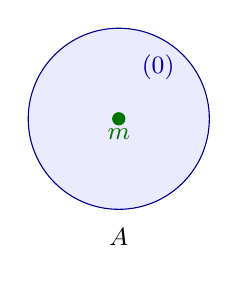
\begin{tikzpicture}[every node/.style={font=\small}]
\filldraw[fill=blue!8,draw=blue!55!black] (0,0) circle (1.15);
\fill[green!45!black] (0,0) circle (2.4pt) node[below] {$\mathfrak m$};
\node[blue!60!black] at (.5,.65) {$(0)$};
\node at (0,-1.5) {$\Spec A$};
\end{tikzpicture}
\end{minipage}\hfill
\begin{minipage}{.63\textwidth}
El centro $\mathfrak m$ es cerrado, con cuerpo residual $\kappa$. El disco sin el centro es $D(\varpi)=\set{(0)}$, con cuerpo residual $K$. Vakil lo llama el germen de una curva. El dibujo representa especializaciones, no un disco con su topología usual. Aquí $\mathbb Z_{(p)}$ es la localización, distinta de la completación $\mathbb Z_p$. \emph{[Vakil, fig.~3.5, \S13.5.5 y \S13.7.]}
\end{minipage}
\end{center}

\begin{prop}[Fibras de $\mathbb P^1_A$ sobre un anillo de valoración discreta]
\label{prop:s09-fibras-dvr}
Sea $A$ un DVR y $\pi:\mathbb P^1_A\to\Spec A$. La fibra genérica $\pi^{-1}((0))$ es abierta y tiene los puntos de $\mathbb P^1_K$; la especial $\pi^{-1}(\mathfrak m)$ es cerrada y tiene los de $\mathbb P^1_{\kappa}$. El primo $(0)$ de $A[t]$ es el punto genérico de $\mathbb P^1_A$. La prueba está en la \cref{prop:s08-fibras-dvr}.
\end{prop}

\section{Reducción de puntos y de ecuaciones}
\emph{Qué buscamos.} Llevar un punto de $\mathbb P^1_K$ a $\mathbb P^1_{\kappa}$. \emph{Idea.} Usar coordenadas en $A$ que no estén ambas en $\mathfrak m$ y reducirlas; dos representantes así difieren por una unidad.

\begin{defi}[Pares normalizados y reducción de un punto]
\label{defi:s09-reduccion-punto}
Un par $(a,b)\in K^2\setminus\set{(0,0)}$ es normalizado si $a,b\in A$ y al menos una coordenada es unidad, es decir, $\min(v(a),v(b))=0$. La reducción de $[a:b]\in\mathbb P^1(K)$ es $[\bar a:\bar b]\in\mathbb P^1(\kappa)$, usando un par normalizado y reduciendo módulo $\mathfrak m$. \emph{[Liu, \S10.1.3, lema~1.32, cor.~1.34 y obs.~1.33 y 1.35; esta última vale para $\mathbb Z_{(p)}$, que no es henseliano.]}
\end{defi}

\begin{lema}[La reducción está bien definida]
\label{lema:s09-reduccion-bien-definida}
Todo punto tiene un representante normalizado, y dos representantes normalizados difieren por una unidad de $A$. Por ello su reducción no depende del representante. \emph{[Liu, \S10.1.3, obs.~1.33.]}
\end{lema}
\begin{proof}
Sea $n=\min(v(a),v(b))$, finito porque el par no es nulo. Multiplicar por $\varpi^{-n}$ normaliza el par. Si $(a',b')=\lambda(a,b)$ y ambos están normalizados, entonces $0=v(\lambda)+0$, de modo que $\lambda\in A^\times$. Sus reducciones son pares no nulos que difieren por $\bar\lambda\in\kappa^\times$.
\end{proof}

\begin{prop}[La cerradura de un punto racional corta la fibra especial en su reducción]
\label{prop:s09-cerradura-reduccion}
Si $(a,b)$ está normalizado y $x$ es el punto de la fibra genérica correspondiente a $[a:b]$, la cerradura $\overline{\set{x}}$ en $\mathbb P^1_A$ corta la fibra especial en exactamente $[\bar a:\bar b]$. La demostración en dos casos, según que $a$ sea unidad o no, está en la \cref{prop:s08-cerradura-reduccion}. \emph{[Liu, \S10.1.3, lema~1.32, cor.~1.34 y obs.~1.35.]}
\end{prop}

\begin{obs}[Existencia de la reducción en general]
\label{obs:s09-reduccion-propiedad}
El morfismo $\mathbb P^n_A\to\Spec A$ es propio y de tipo finito sobre el anillo noetheriano $A$, nociones de las Sesiones 13 a 15. Por el criterio valuativo de propiedad, todo morfismo $\Spec K\to\mathbb P^n_A$ sobre $\Spec A$ se extiende de manera única a $\Spec A\to\mathbb P^n_A$. En $\mathbb P^1$, si $a$ es unidad la extensión está en $U_0$ con $t=b/a$; si no lo es, $b$ es unidad y está en $U_1$ con $s=a/b$. La imagen del punto cerrado es $[\bar a:\bar b]$, la reducción de la \cref{defi:s09-reduccion-punto}. \emph{[Vakil, teos.~11.4.5 y 13.7.6.]}
\end{obs}

% Beamer S09a, diapositiva 10: la cerradura y sus dos puntos en las fibras.
\begin{center}
\begin{tikzpicture}[every node/.style={font=\small}]
\draw[grisCIMAT,->] (-.6,0)--(5.6,0) node[right] {$\Spec A$};
\draw[blue!65!black,thick] plot[domain=.35:3,samples=70] ({.05*sin(900*\x)},\x);
\draw[green!45!black,thick] (4,.35)--(4,3);
\fill[blue!65!black] (0,0) circle (2pt) node[below] {$(0)$};
\fill[green!45!black] (4,0) circle (2pt) node[below] {$\mathfrak m$};
\node[above,blue!65!black] at (0,3) {$\mathbb P^1_K$};
\node[above,green!45!black] at (4,3) {$\mathbb P^1_\kappa$};
\draw[orange!80!black,thick,->] (0,1.9) .. controls (1.4,2.6) and (2.6,2.6) .. (4,1.9);
\fill[orange!80!black] (0,1.9) circle (2.4pt) node[left] {$[a:b]$};
\fill[orange!80!black] (4,1.9) circle (2.4pt) node[right] {$[\bar a:\bar b]$};
\end{tikzpicture}
\end{center}
Para $A=k[u]_{(u)}$, el dibujo se lee como el límite cuando $u\to0$.

\emph{Qué buscamos.} Reducir también la ecuación de un punto. \emph{Idea.} El homomorfismo $A\to\kappa$ lleva ceros de una forma normalizada a ceros de su reducción.

\begin{defi}[Formas normalizadas y su reducción]
\label{defi:s09-reduccion-forma}
Una forma binaria $f=\sum_{i=0}^da_iX^{d-i}Y^i$ sobre $A$ es normalizada si algún $a_i$ es unidad. Toda forma no nula sobre $K$ tiene un múltiplo normalizado $\varpi^{-n}f$, con $n=\min_i v(a_i)$. Dos múltiplos normalizados $f$ y $\lambda f$ difieren por una unidad, pues $0=v(\lambda)+0$. Su reducción es
\[
\bar f=\sum_{i=0}^d\bar a_iX^{d-i}Y^i\in\kappa[X,Y],
\]
una forma no nula de grado $d$. Además, $\overline{\lambda f}=\bar\lambda\bar f$ tiene los mismos ceros que $\bar f$. \emph{[Liu, \S10.1.1, ej.~1.4 y \S10.1.2, def.~1.18.]}
\end{defi}

\begin{prop}[La reducción lleva ceros en ceros]
\label{prop:s09-reduccion-ceros}
Sea $f$ normalizada de grado $d$ sobre $A$, y sea $[a:b]$ un cero con $(a,b)$ normalizado. Entonces $[\bar a:\bar b]$ es cero de $\bar f$. En particular, la forma $bX-aY$ es normalizada, tiene como único cero a $[a:b]$ y se reduce a $\bar bX-\bar aY$, cuyo único cero es $[\bar a:\bar b]$. \emph{[Cálculo elemental; Liu, \S10.1.3, lema~1.32 y obs.~1.35.]}
\end{prop}
\begin{proof}
Reducir $f(a,b)=0$ da $\bar f(\bar a,\bar b)=0$. El par reducido no es nulo por normalización. Para la forma lineal, alguno de sus dos coeficientes es unidad y $bX-aY=0$ expresa la proporcionalidad con $(a,b)$. Lo mismo vale tras reducir.
\end{proof}

\begin{ejem}[El punto $1/2$ y la reducción en cada primo]
\label{ejem:s09-reduccion-medio}
El punto $t=1/2$ es $[2:1]$, con ecuación $X-2Y$; su par es normalizado en $\mathbb Z_{(p)}$ para todo $p$. Si $p$ es impar, se reduce a $[2:1]$, es decir, $t=2^{-1}$ en $\mathbb F_p$. Si $p=2$, la ecuación se reduce a $X$ y el punto a $[0:1]=\infty$. El representante $[1:1/2]$ no sirve en $p=2$, pues $1/2\notin\mathbb Z_{(2)}$.

La presentación compara también $t=3/4=[4:3]$. Los pares con coordenadas enteras coprimas son normalizados en todo primo:
\begin{center}
\small
\renewcommand{\arraystretch}{1.2}
\begin{tabular}{ccccc}
\hline
Punto & $p=2$ & $p=3$ & $p=5$ & $p=7$\\
\hline
$t=1/2=[2:1]$ & $\infty$ & $t=2$ & $t=3$ & $t=4$\\
$t=3/4=[4:3]$ & $\infty$ & $[1:0]$, $t=0$ & $t=2$ & $t=6$\\
\hline
\end{tabular}
\end{center}
\end{ejem}

\begin{ejem}[Dos puntos con la misma reducción, $t=0$ y $t=p$]
\label{ejem:s09-misma-reduccion}
Sobre $A=\mathbb Z_{(p)}$, los puntos $[1:0]$ y $[1:p]$ están normalizados y se reducen al mismo $[1:0]\in\mathbb P^1(\mathbb F_p)$. Sus ecuaciones $-Y$ y $pX-Y$ se reducen ambas a $-Y$. Sus cerraduras $V(t)$ y $V(t-p)$ en $\mathbb P^1_{\mathbb Z}$ se cortan en $V(t,t-p)=V(t,p)$, el punto $(p,t)$. En un primo $q\ne p$, las reducciones son distintas porque la clase de $p$ en $\mathbb F_q$ no es nula. Para $p=2$ es la intersección de las secciones de la \cref{prop:s08-secciones-cero-dos}. \emph{[Liu, \S10.1.3, lema~1.32.]}
\end{ejem}

\section{Los primos sobre \texorpdfstring{$(0)$ y sobre $\mathfrak m$}{(0) y sobre m}}
\label{sec:s09-primos-sobre-base}

\begin{obs}[Lo que se aplaza]
\label{obs:s09-lo-que-se-aplaza}
La definición de modelo usa fibras, productos fibrados y morfismos propios y planos; se retomará cuando el curso disponga de esas nociones. Las fibras de un morfismo son de la Sesión 12, los productos fibrados de la 14 y los morfismos propios de la 15; la planitud y los morfismos étale quedan para un segundo curso. Los cálculos siguientes emplean solo primos, contracción, localización y cocientes. El \cref{sec:s09-modelos} conserva el anticipo sobre modelos y buena reducción, con este alcance.
\end{obs}

\emph{Qué buscamos.} Repartir los primos de $B$ entre los que contraen a $(0)$ y los que contraen a $\mathfrak m$. \emph{Idea.} El espectro de un DVR tiene dos puntos y cada primo de $B$ contrae a uno de ellos.

\begin{prop}[Los primos sobre $(0)$ y sobre $\mathfrak m$]
\label{prop:s09-primos-sobre-dvr}
Sea $A$ un DVR con uniformizante $\varpi$, cuerpo de fracciones $K$ y $\varphi:A\to B$ un homomorfismo. Escribimos también $\varpi$ para $\varphi(\varpi)$. Para un primo $P$ de $B$:
\begin{enumerate}[label=(\alph*)]
\item $\varphi^{-1}(P)=(0)$ si y solo si $\varpi\notin P$, y $\varphi^{-1}(P)=\mathfrak m$ si y solo si $\varpi\in P$. Por tanto $\Spec B$ es la unión disjunta, como conjunto, del abierto $D(\varpi)$ y el cerrado $V(\varpi)$.
\item Los espacios $D(\varpi)$ y $\Spec B[\varpi^{-1}]$ son homeomorfos. Este anillo es la localización de $B$ en las imágenes $\varphi(s)$ con $s\in A\setminus\set{0}$.
\item $V(\varpi)\cong\Spec(B/\mathfrak mB)$ como espacios topológicos.
\end{enumerate}
\emph{[Cálculo elemental; \cref{prop:s09-estructura-dvr}, la correspondencia para localizaciones de la \cref{teo:s03-correspondencia-localizaciones} y la \cref{prop:s09-primos-cociente}.]}
\end{prop}
\begin{proof}
La contracción $\varphi^{-1}(P)$ es un primo de $A$, luego es $(0)$ o $\mathfrak m=(\varpi)$; es el segundo exactamente cuando contiene a $\varpi$. Esto da (a). Todo $s\in A\setminus\set{0}$ es $u\varpi^n$ con $u$ unidad y $n\ge0$, por la \cref{prop:s09-estructura-dvr}. Como $\varphi(u)$ es unidad, invertir las imágenes de todos los $s\ne0$ equivale a invertir $\varpi$. La identificación del abierto básico da (b), incluso si la localización es el anillo cero. Finalmente $\mathfrak mB=\varpi B$, y la correspondencia de primos del cociente identifica $V(\varpi)$ con $\Spec(B/\mathfrak mB)$, con sus topologías.
\end{proof}

\emph{Qué buscamos.} Leer los primos de una ecuación sobre $A$ como los de la ecuación sobre $K$ y los de su reducción. \emph{Idea.} Invertir $\varpi$ y después comparar con el cociente por $\mathfrak m$.

\begin{prop}[Una ecuación sobre un DVR]
\label{prop:s09-ecuacion-dvr}
Sean $A$ un DVR, $f\in A[x]$ y $B=A[x]/(f)$. Entonces
\[
B[\varpi^{-1}]\cong K[x]/(f),\qquad
B/\mathfrak mB\cong\kappa[x]/(\bar f),
\]
donde $\bar f$ reduce coeficiente a coeficiente módulo $\mathfrak m$. Los primos de $B$ que contraen a $(0)$ corresponden a los de $K[x]/(f)$, y los que contraen a $\mathfrak m$ a los de $\kappa[x]/(\bar f)$. \emph{[Cálculo elemental; \cref{prop:s09-estructura-dvr}(e); Vakil, \S10.3.]}
\end{prop}
\begin{proof}
La localización conmuta con el cociente y con el anillo de polinomios, por lo que
\[
(A[x]/(f))[\varpi^{-1}]
\cong A[\varpi^{-1}][x]/(f)=K[x]/(f).
\]
Por otra parte, cocientar por $\mathfrak mB$ equivale a cocientar $A[x]$ por $(f)+\mathfrak mA[x]$. Al reducir los coeficientes queda $\kappa[x]/(\bar f)$. Las correspondencias de la \cref{prop:s09-primos-sobre-dvr} dan la descripción de los primos.
\end{proof}

\begin{ejem}[$x(x-1)$ y $x(x-p)$ sobre $\mathbb Z_{(p)}$]
\label{ejem:s09-ecuaciones-dos-puntos}
Sea $A=\mathbb Z_{(p)}$, con $K=\mathbb Q$ y $\kappa=\mathbb F_p$.
\begin{center}
\small
\setlength{\tabcolsep}{4pt}
\renewcommand{\arraystretch}{1.25}
\begin{tabular}{cllcc}
\hline
$f$ & $\mathbb Q[x]/(f)$ & $\mathbb F_p[x]/(\bar f)$ & \shortstack{Sobre\\$(0)$} & \shortstack{Sobre\\$(p)$}\\
\hline
$x(x-1)$ & $\mathbb Q\times\mathbb Q$ & $\mathbb F_p\times\mathbb F_p$ & dos & dos\\
$x(x-p)$ & $\mathbb Q\times\mathbb Q$ & $\mathbb F_p[x]/(x^2)$ & dos & \shortstack{uno, anillo\\no reducido}\\
\hline
\end{tabular}
\end{center}
En $\mathbb Q[x]$, las parejas $(x),(x-1)$ y $(x),(x-p)$ son comaximales, pues $1=x-(x-1)$ y $1=p^{-1}(x-(x-p))$. La \cref{prop:s09-productos-chino} da $\mathbb Q[x]/(f)\cong\mathbb Q\times\mathbb Q$ en ambas filas. En $\mathbb F_p[x]$, los factores $x$ y $x-1$ siguen siendo comaximales porque $0\ne1$, y dan dos primos.

En cambio, $x(x-p)$ se reduce a $x^2$. Su cociente es $\mathbb F_p[\varepsilon]/(\varepsilon^2)$, cuyo único primo es $(\varepsilon)$: todo primo contiene al nilpotente $\varepsilon$, y el cociente por este ideal es $\mathbb F_p$. La clase $\varepsilon\ne0$ cumple $\varepsilon^2=0$. Es el \cref{ejem:s09-misma-reduccion}: dos puntos distintos se reducen al mismo, y el anillo de la ecuación reducida conserva un nilpotente no nulo. \emph{[Cálculo elemental con la \cref{prop:s09-ecuacion-dvr}; Vakil, \S10.3.]}
\end{ejem}

\emph{Qué buscamos.} Clasificar los primos de $\mathbb Z[i]$ sobre cada primo de $\mathbb Z$. \emph{Idea.} Pasar al cociente $\mathbb Z[i]/(p)$.

\begin{ejem}[{Los primos de $\mathbb Z[i]$ sobre cada primo de $\mathbb Z$}]
\label{ejem:s09-enteros-gaussianos}
Sea $B=\mathbb Z[t]/(t^2+1)$. Evaluar $t\mapsto i$ da $B\cong\mathbb Z[i]$: el mapa es sobreyectivo y el resto de dividir entre el mónico $t^2+1$ es $at+b$, que se anula en $i$ solo si $a=b=0$. Para un primo $P$ de $\mathbb Z[i]$, la contracción $P\cap\mathbb Z$ es $(0)$ o $(p)$ con $p$ primo.
\begin{enumerate}[label=(\alph*)]
\item Sobre $(0)$ solo está $(0)$.
\item Los primos sobre $(p)$ son los que contienen a $p$ y corresponden a los primos del cociente
\[
\mathbb Z[i]/(p)\cong\mathbb F_p[t]/(t^2+1).
\]
\item Según $p$, los anillos son los de la tabla siguiente. En la primera y la última fila hay un primo; en la fila intermedia hay dos.
\end{enumerate}
\begin{center}
\small
\renewcommand{\arraystretch}{1.25}
\begin{tabular}{cll}
\hline
$p$ & Factorización de $t^2+1$ & $\mathbb Z[i]/(p)$\\
\hline
$2$ & $(t+1)^2$ & $\mathbb F_2[\varepsilon]/(\varepsilon^2)$, no reducido\\
$p\equiv1\pmod4$ & $(t-i)(t+i)$, $i^2=-1$ en $\mathbb F_p$ & $\mathbb F_p\times\mathbb F_p$, dos puntos\\
$p\equiv3\pmod4$ & irreducible & $\mathbb F_{p^2}$, un punto de grado $2$\\
\hline
\end{tabular}
\end{center}
\emph{[Cálculo elemental; Vakil, \S10.3, ej.~10.3.4 y 10.3.D.]}
\end{ejem}
\begin{proof}
Si $0\ne z=a+bi\in P$, también $z\bar z=a^2+b^2$ pertenece a $P\cap\mathbb Z$ y es un entero no nulo. Por tanto la contracción solo puede ser $(0)$ cuando $P=(0)$; este ideal sí es primo porque $\mathbb Z[i]$ es dominio.

Contener a $p$ equivale a que la contracción contenga al máximo $(p)$ de $\mathbb Z$, luego a que sea exactamente $(p)$. La \cref{prop:s09-primos-cociente} da la correspondencia de (b). Para $p=2$, poniendo $\varepsilon=t+1$ se obtiene el primer cociente. Si $p\equiv1\pmod4$, la \cref{prop:s09-menos-uno-cuadrado} da dos raíces distintas y el teorema chino da el producto. Si $p\equiv3\pmod4$, no hay raíces y el cuadrático es irreducible, así que el cociente es $\mathbb F_{p^2}$.
\end{proof}

% Beamer S09a, diapositiva 19: V(t^2+1) y la fibra doble.
\par\noindent\begin{minipage}{\linewidth}
\begin{center}
\begin{tikzpicture}[every node/.style={font=\small},x=.95cm]
\draw[grisCIMAT,->] (-.6,0)--(10.2,0) node[right] {$\Spec\mathbb Z$};
\draw[blue!60!black,thick] plot[domain=.3:2.8,samples=75] ({.045*sin(1000*\x)},\x);
\fill[grisCIMAT] (0,0) circle (2pt) node[below] {$(0)$};
\foreach \x/\p in {2/2,4/3,6/5,8/7}{
 \draw[green!45!black] (\x,.3)--(\x,2.8);
 \fill[grisCIMAT] (\x,0) circle (2pt) node[below] {$(\p)$};}
\draw[orange!75!black,thick] (-.4,2.3)--(2,1.8)--(4,1.8)--(6,2.25)--(8,1.8)--(9.5,2.25) node[right] {$\Spec\mathbb Z[i]$};
\draw[orange!75!black,thick] (-.4,1.3)--(2,1.8)--(4,1.8)--(6,1.35)--(8,1.8)--(9.5,1.35);
\draw[orange!75!black,fill=white,thick] (1.94,1.74) rectangle (2.06,1.86);
\fill[orange!75!black] (4,1.8) circle (4pt);
\fill[orange!75!black] (8,1.8) circle (4pt);
\fill[orange!75!black] (6,2.25) circle (2.4pt);
\fill[orange!75!black] (6,1.35) circle (2.4pt);
\node at (9.3,.3) {$\cdots$};
\end{tikzpicture}
\end{center}
El cuadrado marca el único punto doble sobre $2$; los puntos grandes sobre $3$ y $7$ tienen grado $2$, y sobre $5$ hay dos de grado $1$.
\end{minipage}\par

\begin{obs}[Qué se lee de la tabla]
\label{obs:s09-lectura-cociente-gaussiano}
El primo $(0)$ es el único de $\mathbb Z[i]$ que está sobre $(0)$ y es el genérico de su espectro. Los puntos sobre $3$ y $7$ tienen cuerpo residual $\mathbb F_{p^2}$, y los dos sobre $5$ tienen cuerpo residual $\mathbb F_p$.

Sobre $2$, la clase de $1+i$ no es nula: si lo fuera, $(1+i)/2=1/2+i/2$ estaría en $\mathbb Z[i]$. Sin embargo, $(1+i)^2=2i$ se anula módulo $2$. Así $\mathbb Z[i]/(2)$ no es reducido, aunque $\mathbb Z[i]$ es dominio. Este cociente motiva la \cref{defi:s09-esquema-reducido}.
\end{obs}

\section{Modelos y buena reducción}
\label{sec:s09-modelos}
Este apartado recoge el anticipo de modelos y buena reducción. Las nociones aplazadas se precisan en la \cref{obs:s09-lo-que-se-aplaza}; los cálculos de primos anteriores no dependen de ellas.

\emph{Qué buscamos.} Definir la buena reducción de un esquema propio sobre $K$ y calcular ejemplos. \emph{Idea.} Una reducción es la fibra especial de un modelo; la buena reducción exige que algún modelo sea liso.

\begin{defi}[Modelo y reducción]
\label{defi:s09-modelo}
Sea $A$ un DVR y $X$ un esquema propio sobre $K$, no vacío. Un modelo de $X$ sobre $A$ es un esquema $\mathcal X$ plano y propio sobre $\Spec A$, junto con un isomorfismo $\mathcal X_\eta\cong X$ de su fibra genérica. Su imagen es cerrada por propiedad y contiene al genérico $(0)$; como este es denso, $\mathcal X\to\Spec A$ es sobreyectivo. La fibra especial $\mathcal X_s$ se llama una reducción de $X$. Si $\mathcal X=\Spec B$ es afín,
\[
\mathcal X_\eta=\Spec(B\otimes_AK),\qquad
\mathcal X_s=\Spec(B/\mathfrak mB).
\]
La reducción depende fuertemente del modelo. La condición de propiedad excluye usar $X$ mismo sobre $A$, con fibra especial vacía. \emph{[Liu, \S10.1.1, def.~1.1 y obs.~1.6, y \S10.1.2, def.~1.18; pide plano y sobreyectivo, y proyectivo para curvas. Para plano, Liu, \S4.3.1, def.~3.1 y Vakil, def.~24.1.6; para propio, Vakil, def.~11.4.1; para la fibra, Vakil, \S10.3.3.]}
\end{defi}

\begin{defi}[Buena reducción]
\label{defi:s09-buena-reduccion}
El esquema $X$ tiene buena reducción en $A$ si admite un modelo liso sobre $\Spec A$, y mala reducción en otro caso. Liu lo define para curvas proyectivas normales; aquí se emplea la misma definición para esquemas propios, como extensión de estas notas.

La noción de morfismo liso se estudiará más adelante. Vakil define un morfismo liso de dimensión relativa $n$ localmente mediante abiertos de
\[
\Spec B[x_1,\ldots,x_{n+r}]/(f_1,\ldots,f_r)
\]
donde el determinante jacobiano de las $f_j$ respecto de las primeras $r$ variables es invertible; llama étale al caso $n=0$. Liu lo define como plano con fibras lisas y señala que un morfismo étale de tipo finito es liso de dimensión relativa $0$. Que un modelo no sea liso no implica que $X$ tenga mala reducción. \emph{[Liu, \S10.1.2, def.~1.19, obs.~1.6 y \S4.3, def.~3.35; Vakil, def.~13.6.2, ej.~24.8.C--24.8.D y teo.~24.8.8 para la equivalencia de las definiciones de étale.]}
\end{defi}

\begin{ejem}[Un modelo no liso con buena reducción]
\label{ejem:s09-modelos-cubica}
Sea $p\ne3$ primo y sea la curva
\[
C=V(x^3+y^3+p^3z^3)\subseteq\mathbb P^2_{\mathbb Q}.
\]
El modelo con la misma ecuación sobre $\mathbb Z$ tiene reducción $x^3+y^3=0$ en $\mathbb F_p$, singular en $(0:0:1)$: allí se anulan las parciales $3x^2$, $3y^2$ y $0$.

El cambio $w=pz$ da otro modelo
\[
\Proj\mathbb Z[x,y,w]/(x^3+y^3+w^3).
\]
Al invertir $p$ se recupera la ecuación original. Es proyectivo e integral: el polinomio es irreducible en el dominio de factorización única $\mathbb Z[x,y,w]$, su cociente graduado es un dominio y esto se lee en las cartas $D_+(x)$, $D_+(y)$ y $D_+(w)$. Es plano sobre $\mathbb Z$ por ser integral y no constante sobre un esquema de Dedekind. Sobre $\mathbb F_p$ y $\mathbb Q$, las parciales $3x^2$, $3y^2$ y $3w^2$ solo se anulan juntas en $(0:0:0)$. Por el criterio de Jacobi las fibras son lisas; el modelo es liso sobre $\mathbb Z_{(p)}$ y $C$ tiene buena reducción en $p$. \emph{[Liu, \S10.1.2, ej.~1.20; \S4.2.2, teo.~2.19; \S4.3.1, cor.~3.10; \S4.1, def.~1.2.]}
\end{ejem}

\begin{obs}[Resultados generales de Liu, sin demostración]
\label{obs:s09-resultados-liu}
Sea $C$ una curva proyectiva lisa de género $g\ge1$ sobre el cuerpo de fracciones de un esquema de Dedekind $S$ de dimensión $1$. Tiene buena reducción salvo en finitos puntos de $S$. La curva $x^4+y^4+z^4=0$ sobre $\mathbb Q$ tiene buena reducción en $p\ne2$ y mala en $2$. Una curva elíptica tiene buena reducción en $s$ si y solo si el discriminante de su modelo de Weierstrass minimal es unidad en $\mathcal O_{S,s}$. Para variedades abelianas está el criterio de Néron--Ogg--Shafarevich, con referencia a Serre--Tate. Es una observación de lectura, no usada después, con la terminología de Liu. \emph{[Liu, \S10.1.1, ej.~1.12; \S10.1.2, prop.~1.21(a), ej.~1.22 y cor.~1.23; \S10.2.3, obs.~2.34; para Dedekind, \S4.1, def.~1.2.]}
\end{obs}

\emph{Qué buscamos.} Calcular las fibras de un modelo de dimensión cero y decidir cuándo es étale. \emph{Idea.} Reducir $f$ y comprobar dónde su derivada es invertible.

\begin{prop}[Modelos de dimensión cero]
\label{prop:s09-modelos-dimension-cero}
Sea $f\in A[t]$ mónico y $B=A[t]/(f)$, libre como $A$-módulo y por ello plano.
\begin{enumerate}[label=(\alph*)]
\item Para $\mathfrak p\in\Spec A$, la fibra es $\Spec\kappa(\mathfrak p)[t]/(\bar f)$. Si $A$ es un DVR, $B\otimes_AK=K[t]/(f)$ y $B/\mathfrak mB=\kappa[t]/(\bar f)$.
\item El morfismo $\Spec B\to\Spec A$ es étale en los puntos donde $f'$ es invertible.
\item Si $A$ es un DVR, es étale en toda la fibra especial si y solo si $\bar f$ es separable, es decir, no tiene raíces múltiples en una clausura algebraica de $\kappa$.
\end{enumerate}
\emph{[Vakil, def.~13.6.2 y ej.~24.8.C--24.8.D; Liu, \S4.3.2, def.~3.17, lema~3.20 y ej.~3.21.]}
\end{prop}
\begin{proof}
La división entre el mónico $f$ da la base $1,t,\ldots,t^{d-1}$ de $B$ sobre $A$. Cambiar escala a $\kappa(\mathfrak p)$ reduce sus coeficientes y da (a). Para (b), el jacobiano de la presentación con una variable y una ecuación es $f'$: donde se invierte, la presentación es étale por el criterio recordado en la \cref{defi:s09-buena-reduccion}.

En la fibra especial, la condición es que $\bar f'$ sea unidad en $\kappa[t]/(\bar f)$, equivalente a $(\bar f,\bar f')=(1)$ en $\kappa[t]$. Esto equivale a que $\bar f$ no tenga raíces múltiples. Si hay una raíz múltiple en la clausura algebraica, el punto correspondiente de la fibra tiene derivada nula y el modelo no es étale allí, por el criterio de Liu citado. Esto prueba ambas implicaciones de (c).
\end{proof}

\begin{lema}[Discriminante de un polinomio mónico de grado $2$]
\label{lema:s09-discriminante-cuadratico}
Sea $F$ un cuerpo y sea $f=t^2+bt+c$ en $F[t]$. Sus dos raíces en una clausura algebraica son distintas si y solo si $b^2-4c\ne0$. Si $f\in A[t]$ con $A$ un DVR, $\bar f$ es separable si y solo si $b^2-4c\in A^\times$.
\end{lema}
\begin{proof}
Si $r_1,r_2$ son las raíces, $b=-(r_1+r_2)$ y $c=r_1r_2$, luego $b^2-4c=(r_1-r_2)^2$ en cualquier característica. Este elemento es no nulo si y solo si las raíces son distintas. El discriminante de $\bar f$ es la reducción del discriminante de $f$, que es no nula si y solo si este no está en $\mathfrak m$, es decir, si es unidad.
\end{proof}

\emph{El modelo de los enteros gaussianos.} El anillo del \cref{ejem:s09-enteros-gaussianos} da el modelo de $\Spec\mathbb Q(i)$ de la \cref{prop:s09-modelos-dimension-cero}. La fibra genérica tiene anillo $\mathbb Q[t]/(t^2+1)=\mathbb Q(i)$. El discriminante es $-4$, unidad en $\mathbb Z_{(p)}$ si y solo si $p$ es impar. Por tanto el modelo es étale sobre $\mathbb Z_{(p)}$ para todo primo impar y $\Spec\mathbb Q(i)$ tiene buena reducción allí. Sobre $2$ el modelo no es étale. En los tres casos el anillo de la fibra tiene dimensión $2$ sobre el cuerpo de la base: dos puntos, un punto no reducido o una extensión de grado $2$. \emph{[Vakil, ej.~10.3.4, ej.~10.3.D, \S16.3.10 y \S21.7.1; Liu, \S4.3.2, lema~3.20.]}


En $B$, $t(-t)=1$, de modo que $f'=2t$ es invertible exactamente donde $2$ lo es; esto confirma la afirmación sobre étale y el cálculo del discriminante.

\begin{obs}[El mismo comportamiento sobre un cuerpo]
\label{obs:s09-parabola-vakil}
La proyección de $y^2=x$ sobre el eje $x$ en $\mathbb Q$ tiene dos puntos sobre $x=1$, un punto no reducido $\Spec\mathbb Q[y]/(y^2)$ sobre $x=0$, y un punto con cuerpo residual $\mathbb Q(i)$ sobre $x=-1$. Sobre el genérico hay un punto con cuerpo residual $\mathbb Q(y)$, extensión de grado $2$ de $\mathbb Q(x)$. Es el mismo patrón de la \cref{ejem:s09-enteros-gaussianos}. Vakil señala además que, si $B$ es el anillo de enteros de un cuerpo numérico, su ideal diferente mide la ramificación de $\Spec B\to\Spec\mathbb Z$. \emph{[Vakil, ej.~10.3.4 y 10.3.D, \S16.3.10 y \S21.7.1.]}
\end{obs}

\begin{obs}[Una degeneración a un nodo]
\label{obs:s09-degeneracion-nodo}
La familia $y^2=x^3+x^2+tx$ tiene miembros generales lisos y en $t=0$ da la curva nodal $y^2=x^2(x+1)$, singular en el origen. También es singular el miembro $t=1/4$, donde el discriminante de $x^2+x+t$ se anula y la ecuación es $y^2=x(x+1/2)^2$. \emph{[Vakil, \S24.1, fig.~24.1.]}
\end{obs}

\section{\texorpdfstring{$\mathbb P^n_A$}{PnA} y sus datos de pegado}
\emph{Qué buscamos.} Construir $\mathbb P^n_A$ mediante sus funciones de pegado. \emph{Idea.} Pegar $n+1$ copias de $\mathbb A^n_A$ con cocientes de coordenadas homogéneas.

\begin{defi}[Las cartas de $\mathbb P^n_A$]
\label{defi:s09-cartas-proyectivas}
Para cada índice $i=0,\ldots,n$, ponemos
\[
A_i=A[x_{k/i}:k\ne i],\qquad U_i=\Spec A_i\cong\mathbb A^n_A.
\]
Cada anillo tiene $n$ variables, y $x_{k/i}$ representa $x_k/x_i$. Ponemos $x_{i/i}=1$, $U_{ii}=U_i$ y $\varphi_{ii}=\id$. Si $j\ne i$, sea $U_{ij}=D(x_{j/i})\subseteq U_i$, y definamos $\varphi_{ij}:U_{ij}\to U_{ji}$ por
\[
\varphi_{ij}^\sharp:A_j[x_{i/j}^{-1}]\longrightarrow A_i[x_{j/i}^{-1}],
\qquad x_{k/j}\longmapsto\frac{x_{k/i}}{x_{j/i}}\quad(k\ne j).
\]
En particular, $x_{i/j}\mapsto x_{j/i}^{-1}$. \emph{[Vakil, \S4.4.9--4.4.10; \cref{defi:s08-cartas-proyectiva-n}.]}
\end{defi}

\begin{ejem}[$\mathbb P^2_A$]
\label{ejem:s09-pegados-plano-proyectivo}
Las tres cartas y sus coordenadas son
\[
\begin{aligned}
U_0&=\Spec A[u,v], &(u,v)&=(x_1/x_0,x_2/x_0),\\
U_1&=\Spec A[u',v'], &(u',v')&=(x_0/x_1,x_2/x_1),\\
U_2&=\Spec A[u'',v''], &(u'',v'')&=(x_0/x_2,x_1/x_2).
\end{aligned}
\]
Los pegados son
\[
\begin{aligned}
\varphi_{01}:D(u)&\longrightarrow D(u'), &(u,v)&\longmapsto(1/u,v/u),\\
\varphi_{02}:D(v)&\longrightarrow D(u''), &(u,v)&\longmapsto(1/v,u/v),\\
\varphi_{12}:D(v')&\longrightarrow D(v''), &(u',v')&\longmapsto(u'/v',1/v').
\end{aligned}
\]
Para $n=1$ se recupera $\mathbb P^1_A$ con $t=x_{1/0}$ y $s=x_{0/1}$. En el traslape triple del plano, el cociclo es la identidad de funciones racionales
\[
\varphi_{12}(\varphi_{01}(u,v))
=\varphi_{12}(1/u,v/u)=(1/v,u/v)=\varphi_{02}(u,v).
\]
\end{ejem}

\begin{prop}[$\mathbb P^n_A$]
\label{prop:s09-pegado-proyectivo}
Los $U_i,U_{ij},\varphi_{ij}$ de la \cref{defi:s09-cartas-proyectivas} son datos de pegado, incluida $\varphi_{ij}(U_{ij}\cap U_{ik})=U_{ji}\cap U_{jk}$. Su pegado es $\mathbb P^n_A$. La prueba con el anillo $L_0$ de monomios de grado cero está en la \cref{prop:s08-cociclo-proyectiva-n}. El \cref{ejem:s09-pegados-plano-proyectivo} verifica el cociclo para $n=2$, y los inversos se piden en el \cref{ejer:s09-pegados-inversos}. \emph{[Vakil, \S4.4.9--4.4.10 y ej.~4.4.D.]}
\end{prop}

\begin{obs}
\label{obs:s09-proyectivo-modelo-liso}
La carta $U_0\cong\mathbb A^n_A$ es abierta y su complemento es el hiperplano $x_0=0$, que se identificará con $\mathbb P^{n-1}_A$ en la Sesión 10. En el plano, es $V(u')$ en $U_1$ y $V(u'')$ en $U_2$. Las fibras sobre $\mathfrak p$ son $\mathbb P^n_{\kappa(\mathfrak p)}$.

Liu afirma que $\mathbb P^n_{\mathbb Z}$ es liso sobre $\Spec\mathbb Z$; los morfismos lisos son estables por cambio de base, así que $\mathbb P^n_A$ es un modelo liso de $\mathbb P^n_K$ sobre todo DVR $A$. La construcción sistemática como $\Proj$ llega en la Sesión 21. \emph{[Liu, \S4.2, ej.~2.13 y \S4.3, ej.~3.37 y prop.~3.38.]}
\end{obs}

\section{Resultados de las sesiones 9a y 9b}

Los DVR de la \cref{defi:s09-dvr} dan ejemplos de esquemas integrales y noetherianos. El \cref{ejem:s09-enteros-gaussianos} calcula los primos de $\mathbb Z[i]$ sobre cada primo de $\mathbb Z$ y da el ejemplo de un cociente no reducido sobre $2$. Las cartas de la \cref{defi:s09-cartas-proyectivas} y su pegado en la \cref{prop:s09-pegado-proyectivo} permiten estudiar las propiedades de $\mathbb P^n_A$ a partir de sus abiertos afines.

\section{Propiedades básicas de esquemas}
\subsection{Qué buscamos}

\begin{obs}[Qué buscamos]
\label{obs:s09-cuatro-propiedades}
Aunque $\mathbb Z[i]$ es un dominio, el anillo de la fibra sobre $2$ tiene un nilpotente no nulo. La fibra sobre $5$ consta de dos puntos. Ambos cálculos, en el \cref{ejem:s09-enteros-gaussianos}, motivan las dos primeras propiedades.
\begin{enumerate}
\item \emph{Reducido.} Ningún tallo tiene nilpotentes no nulos; falla en $\Spec k[\varepsilon]/(\varepsilon^2)$.
\item \emph{Irreducible.} El espacio tiene una sola pieza. Los ejes de $\Spec k[x,y]/(xy)$ son dos componentes irreducibles.
\item \emph{Integral.} Reducido e irreducible. Sus anillos de secciones sobre abiertos no vacíos son dominios y el esquema tiene un cuerpo de funciones.
\item \emph{Noetheriano.} Admite un cubrimiento afín finito por espectros de anillos noetherianos y tiene finitas componentes irreducibles.
\end{enumerate}
Aplicaremos los cuatro adjetivos a los ejemplos guía y a los cocientes de $\mathbb Z[i]$ por un primo en los \cref{ejem:s09-tabla-propiedades,ejem:s09-adjetivos-fibras}. \emph{[Vakil, \S5.1--5.3, ej.~3.2.A(a) y 3.7.I; Liu, \S2.3.4 y \S2.4.]}
\end{obs}

\subsection{Reducido}
\emph{Qué buscamos.} Decir cuándo un esquema no tiene nilpotentes y reducir la pregunta a abiertos afines.

\begin{defi}[Esquema reducido]
\label{defi:s09-esquema-reducido}
Un esquema $X$ es reducido si todos sus tallos $\mathcal O_{X,x}$ son reducidos. \emph{[Vakil, \S5.2.1; Liu, def.~4.1.]}
\end{defi}

\emph{Qué buscamos.} Calcular los tallos de un afín reducido. \emph{Idea.} Multiplicar el numerador de un nilpotente localizado por un elemento del conjunto multiplicativo.

\begin{lema}[Localización de un anillo reducido]
\label{lema:s09-localizacion-reducida}
Si $A$ es reducido y $S\subseteq A$ es multiplicativo, $S^{-1}A$ es reducido. En particular, lo son $A_{\mathfrak p}$ y $A_f$. \emph{[Cálculo elemental; Atiyah--Macdonald, cap.~3.]}
\end{lema}
\begin{proof}
Si $(a/s)^n=0$, hay $u\in S$ con $ua^n=0$. Entonces $(ua)^n=u^{n-1}(ua^n)=0$. Como $A$ es reducido, $ua=0$, y por la \cref{prop:s09-localizacion} se tiene $a/s=0$.
\end{proof}

\emph{Qué buscamos.} Leer la reducción de un esquema en sus anillos de secciones y en un cubrimiento afín. \emph{Idea.} Un nilpotente nulo en todas las localizaciones tiene un anulador que no está en ningún primo; un germen nilpotente se representa por una sección nilpotente cerca del punto.

\begin{prop}[Reducido en abiertos afines]
\label{prop:s09-reducido-afines}
Sea $X$ un esquema.
\begin{enumerate}[label=(\alph*)]
\item $\Spec A$ es reducido si y solo si $A$ es reducido.
\item $X$ es reducido si y solo si $\mathcal O_X(U)$ es reducido para todo abierto $U$.
\item Si $X$ admite una cubierta por afines $\Spec A_i$ con todos los $A_i$ reducidos, es reducido.
\end{enumerate}
En particular, todo abierto afín de un esquema reducido tiene anillo de secciones reducido. \emph{[Vakil, ej.~5.2.B; Liu, prop.~4.2(a)--(b).]}
\end{prop}
\begin{proof}
Para (a), calculamos en los tallos $A_{\mathfrak p}$.
\par\smallskip\noindent
\begin{tabular}{@{}p{.56\linewidth}p{.40\linewidth}@{}}
\textbf{Qué hacemos} & \textbf{Por qué se vale}\\[2pt]
\hline
$\Rightarrow$ Sea $a^n=0$. Si $\Spec A$ es reducido, $a/1=0$ en cada $A_{\mathfrak p}$, de modo que hay $u\notin\mathfrak p$ con $ua=0$. Así $\operatorname{Ann}(a)=A$ y $a=0$.
& $a/1$ es nilpotente en el tallo reducido. Ningún primo contiene $\operatorname{Ann}(a)$, por lo que se aplica la \cref{prop:s09-maximos-minimales}(a).\\[4pt]
$\Leftarrow$ Si $A$ es reducido, todos los $A_{\mathfrak p}$ son reducidos.
& Es el \cref{lema:s09-localizacion-reducida} aplicado a los tallos.
\end{tabular}
\par\smallskip

Para (b), si $X$ es reducido y $s^n=0$ en $\mathcal O(U)$, todos los gérmenes de $s$ son nulos. Cada punto tiene un entorno donde $s$ se anula y (G1) da $s=0$. Recíprocamente, si todos los anillos de secciones son reducidos y un germen $s_x$ cumple $s_x^n=0$, en algún entorno $V$ se tiene $(s|_V)^n=0$. Entonces $s|_V=0$ y $s_x=0$. Finalmente, en (c) cada tallo se calcula en una carta reducida por (a).
\end{proof}

\emph{Qué buscamos.} Ver qué se pierde en un esquema no reducido.

\begin{ejem}[{$\Spec k[\varepsilon]/(\varepsilon^2)$}]
\label{ejem:s09-numeros-duales}
Sea $A=k[x]/(x^2)=k[\varepsilon]/(\varepsilon^2)$, con $\varepsilon$ la clase de $x$. Su espectro es un solo punto de cuerpo residual $k$, y no es reducido. El anillo $A=\set{a+b\varepsilon\given a,b\in k}$ tiene dimensión $2$ sobre $k$. La función $\varepsilon\ne0$ tiene el mismo valor que la función $0$ en el único punto. \emph{[Vakil, ej.~3.2.A(a), \S3.2.12 y \S3.2.14.]}
\end{ejem}
\begin{proof}
Todo primo contiene a $\varepsilon$ porque contiene a $\varepsilon^2=0$, y $(\varepsilon)$ es máximo con cociente $k$. Así $\Spec A=\set{(\varepsilon)}$. La clase $\varepsilon$ es no nula, aunque su imagen en $A/(\varepsilon)=k$ es cero. Por la \cref{prop:s09-reducido-afines}, el esquema no es reducido.
\end{proof}

% Beamer S09a (24) y S09c (3): un punto con una dirección infinitesimal.
\begin{center}
\begin{tikzpicture}[every node/.style={font=\small}]
\draw[grisCIMAT,dashed] (0,0) ellipse (.65 and .35);
\fill[orange!80!black] (0,0) circle (2.6pt) node[below=8pt] {$(\varepsilon)$};
\draw[->,blue!65!black,thick] (0,.08)--(0,1.25) node[right] {$\varepsilon$};
\end{tikzpicture}
\end{center}

\emph{Qué buscamos.} Saber cuándo una función se determina por sus valores.

\begin{prop}[Funciones y valores]
\label{prop:s09-funciones-valores}
Sea $X$ reducido, $U\subseteq X$ abierto y $s,t\in\mathcal O(U)$ con $s(x)=t(x)$ en $\kappa(x)$ para todo $x\in U$. Entonces $s=t$. El \cref{ejem:s09-numeros-duales} muestra que la hipótesis es necesaria. \emph{[Vakil, ej.~5.2.A.]}
\end{prop}
\begin{proof}
Restamos $t$ y suponemos $s(x)=0$ en cada punto. En un afín $W=\Spec B\subseteq U$, la \cref{prop:s09-tallos-valores-afin} dice que $s|_W$ pertenece a todo primo de $B$, por lo que está en $\Nil(B)=0$. Como estos afines cubren $U$, (G1) da $s=0$.
\end{proof}

\emph{Qué buscamos.} Reconocer esquemas reducidos conocidos.

\begin{ejem}[Ejemplos reducidos]
\label{ejem:s09-reducidos}
\begin{enumerate}[label=(\alph*)]
\item Para $n\ge2$, $\Spec\mathbb Z/n\mathbb Z$ es reducido si y solo si $n$ es producto de primos distintos.
\item Si $A$ es un dominio, $\mathbb A^n_A$ y $\mathbb P^n_A$ son reducidos. En particular, lo son sobre $k$ y sobre $\mathbb Z$.
\end{enumerate}
\emph{[(b) extiende de un cuerpo a un dominio el ej.~5.2.C de Vakil; (a) es cálculo elemental.]}
\end{ejem}
\begin{proof}
Si $n$ es libre de cuadrados, el teorema chino da $\mathbb Z/n\mathbb Z\cong\prod_{p\mid n}\mathbb F_p$, reducido. Si $p^2\mid n$, la clase de $n/p$ es no nula y su cuadrado es divisible por $n$, así que el anillo no es reducido. Para (b), las cartas tienen anillos de polinomios sobre un dominio, por tanto reducidos; aplicamos la \cref{prop:s09-reducido-afines}.
\end{proof}

\begin{obs}
\label{obs:s09-estructura-reducida}
Los anillos no reducidos aparecen al reducir módulo un primo. En el \cref{ejem:s09-enteros-gaussianos}, el cociente $\mathbb Z[i]/(2)$ da el espectro del \cref{ejem:s09-numeros-duales} con $k=\mathbb F_2$. La estructura reducida $X_{\mathrm{red}}$ queda de lectura y se retoma en la Sesión 10. \emph{[Liu, prop.~4.2(c).]}
\end{obs}

\subsection{Irreducible y componentes irreducibles}
\emph{Qué buscamos.} Decir cuándo un espacio tiene una sola pieza y descomponerlo en sus piezas.

\begin{defi}[Espacio irreducible y componentes irreducibles]
\label{defi:s09-irreducible}
Un espacio $X$ es irreducible si $X\ne\varnothing$ y no es unión de dos cerrados propios. Un subconjunto es irreducible con la topología de subespacio; una componente irreducible es un subconjunto irreducible maximal para la inclusión. Un esquema es irreducible si lo es su espacio topológico. \emph{[Vakil, \S3.6.4 y \S3.6.12; Liu, \S2.4.2 y def.~4.6.]}
\end{defi}

\emph{Qué buscamos.} Reconocer irreducibles con abiertos y ver que las componentes son cerradas y cubren el espacio. \emph{Idea.} Pasar a complementos y usar Zorn sobre cadenas de irreducibles.

\begin{lema}[Hechos topológicos sobre irreducibles]
\label{lema:s09-topologia-irreducibles}
\begin{enumerate}[label=(\alph*)]
\item $X$ es irreducible si y solo si es no vacío y dos abiertos no vacíos cualesquiera se cortan.
\item Todo abierto no vacío de un irreducible es denso e irreducible. Todo irreducible es conexo.
\item La cerradura de un subconjunto irreducible es irreducible.
\item Las componentes irreducibles son cerradas y cubren $X$; todo irreducible está contenido en una. Un cerrado irreducible es componente si y solo si es maximal entre los cerrados irreducibles.
\end{enumerate}
\emph{[Liu, \S2.4.2 y prop.~4.5(a); Vakil, ej.~3.6.B, 3.6.D y 3.6.O.]}
\end{lema}
\begin{proof}
La equivalencia (a) resulta de tomar complementos. Para (b), un abierto no vacío $U$ corta todo abierto no vacío de $X$, así que es denso. Dos abiertos no vacíos de $U$ son abiertos de $X$ y se cortan. Una separación de $X$ en abiertos no vacíos contradice (a).

Para (c), dos abiertos de $\overline Y$ no vacíos cortan a $Y$ por densidad; sus trazas en el irreducible $Y$ se cortan. Para (d), la unión de una cadena de irreducibles es irreducible: dados dos abiertos que la cortan, un miembro de la cadena contiene puntos de ambas intersecciones y fuerza que estas se corten. Zorn da un irreducible maximal que contiene a cualquier irreducible dado. Su cerradura es irreducible por (c), así que la maximalidad lo hace cerrado. Como cada punto es irreducible, las componentes cubren $X$; la última afirmación sigue tomando cerraduras.
\end{proof}

\emph{Qué buscamos.} Decidir cuándo $V(I)$ tiene una pieza y leer las componentes en el anillo. \emph{Idea.} Un producto $ab\in\sqrt I$ reparte $V(I)$ entre $V(a)$ y $V(b)$.

\begin{prop}[Cerrados irreducibles de $\Spec A$]
\label{prop:s09-irreducibles-espectro}
\begin{enumerate}[label=(\alph*)]
\item $V(I)$ es irreducible si y solo si $\sqrt I$ es primo; entonces $V(I)=V(\sqrt I)=\overline{\set{\sqrt I}}$.
\item Los cerrados irreducibles son los $V(\mathfrak p)$ con $\mathfrak p$ primo, y $V(\mathfrak p)\subseteq V(\mathfrak q)$ si y solo si $\mathfrak q\subseteq\mathfrak p$.
\item Las componentes de $\Spec A$ son los $V(\mathfrak p)$ con $\mathfrak p$ primo minimal.
\item $\Spec A$ es irreducible si y solo si $\Nil(A)$ es primo, si y solo si hay exactamente un primo minimal. En particular, lo es si $A$ es un dominio.
\end{enumerate}
\emph{[Liu, prop.~4.7; Vakil, ej.~3.6.C, 3.7.F y 3.7.G.]}
\end{prop}
\begin{proof}
Si $\sqrt I=\mathfrak p$ es primo, $V(I)=\overline{\set{\mathfrak p}}$ es irreducible por el \cref{lema:s09-topologia-irreducibles}(c). Recíprocamente, si $V(I)$ es irreducible y $ab\in\sqrt I$, entonces
\[
V(I)=(V(I)\cap V(a))\cup(V(I)\cap V(b)).
\]
Uno de los dos cerrados es todo $V(I)$; si es el primero, $a\in\bigcap_{\mathfrak p\supseteq I}\mathfrak p=\sqrt I$. Además $\sqrt I\ne A$ porque $V(I)\ne\varnothing$. Esto prueba (a).

Para (b), usamos (a) y observamos que $V(\mathfrak p)\subseteq V(\mathfrak q)$ implica $\mathfrak p\in V(\mathfrak q)$, es decir, $\mathfrak q\subseteq\mathfrak p$; la recíproca es inmediata. La inversión de inclusiones da (c). Para (d), aplicamos (a) a $I=(0)$. Si $\Nil(A)$ es primo, está en todos los primos y es el único minimal. Si hay un único minimal $\mathfrak p_0$, todo primo lo contiene por la \cref{prop:s09-maximos-minimales}, luego $\mathfrak p_0=\bigcap\mathfrak p=\Nil(A)$.
\end{proof}
\emph{Advertencia.} Basta que $\sqrt I$ sea primo. En $\Spec k[x]$, el cerrado $V(x^2)=\set{(x)}$ es irreducible, aunque $(x^2)$ no es primo.

\emph{Qué buscamos.} Distinguir conexidad e irreducibilidad con dos ejemplos.

\begin{ejem}[Los dos ejes y $\Spec\mathbb Z/6\mathbb Z$]
\label{ejem:s09-dos-ejes}
Las componentes de $\Spec k[x,y]/(xy)$ son los ejes $V(x)$ y $V(y)$; se cortan en el origen $(\bar x,\bar y)$. El espacio es conexo y no irreducible. En cambio, $\Spec\mathbb Z/6\mathbb Z$ consta de dos puntos $(2)$ y $(3)$, sus componentes, y no es conexo ni irreducible. \emph{[Vakil, ej.~3.6.E, 3.7.I y 3.6.A, y \S3.6.12.]}
\end{ejem}
\begin{proof}
Los primos de $k[x,y]$ que contienen $xy$ contienen $x$ o $y$. Los primos minimales del cociente son $(\bar x)$ y $(\bar y)$, y las componentes son sus cerrados por la \cref{prop:s09-irreducibles-espectro}. Cada eje es una recta afín irreducible y conexa, y ambos contienen el origen; su unión es conexa. Son dos cerrados propios, así que no es irreducible. Finalmente $\mathbb Z/6\mathbb Z\cong\mathbb F_2\times\mathbb F_3$ da los dos puntos abiertos y cerrados del segundo ejemplo.
\end{proof}

% Beamer S09a (32) y S09c (10): los ejes con su punto común.
\begin{center}
\begin{tikzpicture}[every node/.style={font=\small}]
\draw[blue!65!black,thick] (-2,0)--(2,0) node[right] {$V(y)$};
\draw[green!45!black,thick] (0,-1.3)--(0,1.5) node[above] {$V(x)$};
\fill[orange!80!black] (0,0) circle (2.5pt) node[below right] {$(\bar x,\bar y)$};
\end{tikzpicture}
\end{center}

\emph{Qué buscamos.} Ver la irreducibilidad de $\mathbb P^n_A$ a partir de sus cartas.

\begin{lema}[Pegado de irreducibles]
\label{lema:s09-pegado-irreducibles}
Si $X$ está cubierto por abiertos irreducibles $U_i$, hay al menos uno y $U_i\cap U_j\ne\varnothing$ para todo $i,j$, entonces $X$ es irreducible. En particular, si $A$ es un dominio, $\mathbb P^n_A$ es irreducible. También lo son $\mathbb A^n_A$, $\Spec\mathbb Z$ y $\Spec\mathbb Z[t]$. \emph{[Vakil, ej.~5.1.A, extendido de un cuerpo a un dominio.]}
\end{lema}
\begin{proof}
Sean $V,W$ abiertos no vacíos de $X$. Hay $i,j$ con $V\cap U_i\ne\varnothing$ y $W\cap U_j\ne\varnothing$. En $U_i$, los abiertos no vacíos $V\cap U_i$ y $U_i\cap U_j$ se cortan. Así $V\cap U_j\ne\varnothing$, y en el irreducible $U_j$ corta a $W\cap U_j$. Por el \cref{lema:s09-topologia-irreducibles}(a), $X$ es irreducible. Si $A$ es dominio, los anillos de las cartas de $\mathbb P^n_A$ son dominios y los traslapes $D(x_{j/i})$ no son vacíos, porque $x_{j/i}$ no es nilpotente. Los ejemplos afines siguen de la \cref{prop:s09-irreducibles-espectro}(d).
\end{proof}

\emph{Qué buscamos.} Asignar a cada cerrado irreducible un único punto que lo llena. \emph{Idea.} Reducir a una carta afín y recuperar la cerradura desde su traza.

\begin{prop}[Puntos genéricos]
\label{prop:s09-puntos-genericos}
En un esquema $X$, la aplicación $x\mapsto\overline{\set{x}}$ es una biyección entre puntos y cerrados irreducibles. Todo cerrado irreducible tiene un único punto genérico. En particular, un esquema irreducible tiene un único genérico $\eta$, que está en todo abierto no vacío. \emph{[Vakil, ej.~5.1.B; Liu, prop.~4.12(a) para componentes.]}
\end{prop}
\begin{proof}
La cerradura de un punto es irreducible. Sea $Z$ cerrado irreducible y $W=\Spec A$ una carta con $Z\cap W\ne\varnothing$. Esta intersección es densa en $Z$ e irreducible, así que por la \cref{prop:s09-irreducibles-espectro} es $V_W(\mathfrak p)$ para un primo $\mathfrak p$. Si $\xi$ es su punto, $\overline{\set{\xi}}\subseteq Z$ y contiene a $Z\cap W$, luego es $Z$.

Si $\overline{\set{x}}=\overline{\set{y}}$, una carta afín $W$ que contiene a $x$ contiene también a $y$, por la \cref{obs:s09-especializacion-local}. Sus cerraduras en $W$ son iguales, y $V_W(\mathfrak p_x)=V_W(\mathfrak p_y)$ implica $\mathfrak p_x=\mathfrak p_y$. Por tanto $x=y$. La última afirmación sigue de la densidad de $\set{\eta}$.
\end{proof}

\begin{ejem}[Irreducibles conocidos]
\label{ejem:s09-irreducibles-conocidos}
Los esquemas $\mathbb A^n_k$, $\mathbb P^n_k$, $\Spec\mathbb Z$ y $\Spec\mathbb Z[t]$ son irreducibles por el \cref{lema:s09-pegado-irreducibles}; el genérico del último es $(0)$. Todo irreducible es conexo, pero los dos ejes del \cref{ejem:s09-dos-ejes} muestran que la recíproca falla. \emph{[Vakil, ej.~3.6.C--3.6.E y 5.1.A.]}
\end{ejem}

\subsection{Integral}
\emph{Qué buscamos.} Reunir una sola pieza y ausencia de nilpotentes en una noción.

\begin{defi}[Esquema integral]
\label{defi:s09-esquema-integral}
Un esquema $X$ es integral si $X\ne\varnothing$ y $\mathcal O_X(U)$ es un dominio para todo abierto no vacío $U$. \emph{[Vakil, \S5.2.4; Liu, prop.~4.17.]}
\end{defi}

% Beamer S09a (35) y S09c (11): las dos obstrucciones y una curva integral.
\begin{center}
\begin{tikzpicture}[every node/.style={font=\small}]
\draw[grisCIMAT,dashed] (0,0) ellipse (.5 and .25);
\fill[orange!80!black] (0,0) circle (2.4pt);
\draw[->,blue!65!black] (0,.05)--(0,1);
\node[align=center] at (0,-.75) {$\Spec k[\varepsilon]/(\varepsilon^2)$\\no reducido};
\draw[blue!65!black,thick] (2.6,0)--(4.4,0);
\draw[green!45!black,thick] (3.5,-.7)--(3.5,.9);
\fill[orange!80!black] (3.5,0) circle (2.4pt);
\node[align=center] at (3.5,-1.2) {$\Spec k[x,y]/(xy)$\\no irreducible};
\draw[orange!80!black,thick] (6,-.5) .. controls (6.5,.2) and (6.5,.8) .. (7,.4)
 .. controls (7.4,0) and (7.6,.5) .. (8,1);
\node at (7,-.8) {una curva integral};
\end{tikzpicture}
\end{center}

\emph{Qué buscamos.} Equivalencia entre dominios de secciones y reducido e irreducible. \emph{Idea.} Una separación en cerrados da dos abiertos disjuntos y un producto de anillos. Para la recíproca, si $fg=0$, sus lugares de anulación cubren un irreducible.

\begin{prop}[Integral es reducido e irreducible]
\label{prop:s09-integral-equivalencia}
Un esquema es integral si y solo si es reducido e irreducible. \emph{[Vakil, ej.~5.2.G; Liu, def.~4.16 y prop.~4.17.]}
\end{prop}
\begin{proof}
\emph{Integral implica reducido e irreducible.} Los anillos de secciones sobre abiertos no vacíos son dominios y por tanto reducidos; además $\mathcal O(\varnothing)=0$. La \cref{prop:s09-reducido-afines}(b) da que $X$ es reducido. Si $X=Z_1\cup Z_2$ con cerrados propios, los abiertos $U_i=X\setminus Z_i$ son no vacíos y disjuntos. Por (G2),
\[
\mathcal O(U_1\cup U_2)\cong\mathcal O(U_1)\times\mathcal O(U_2).
\]
Ambos factores son no nulos, y $(1,0)(0,1)=0$ contradice que el anillo de secciones del abierto no vacío $U_1\cup U_2$ sea dominio.

\emph{Reducido e irreducible implica integral.} Sea $U\ne\varnothing$ abierto. Probamos que $\mathcal O(U)$ es un dominio.
\par\smallskip\noindent
\begin{tabular}{@{}p{.51\linewidth}p{.45\linewidth}@{}}
\textbf{Qué hacemos} & \textbf{Por qué se vale}\\[2pt]
\hline
Sean $f,g\in\mathcal O(U)$ con $fg=0$. En cada $x\in U$ se tiene $f_xg_x=0$, de modo que $f_x\in\mathfrak m_x$ o $g_x\in\mathfrak m_x$.
& Por (G3), $\mathcal O(U)\ne0$. Los gérmenes no pueden ser ambos unidades, pues $0$ no es una unidad del anillo local $\mathcal O_{X,x}\ne0$.\\[4pt]
Los conjuntos $V_U(f)=\set{x\in U\given f_x\in\mathfrak m_x}$ y $V_U(g)$ son cerrados y cubren $U$. Podemos suponer que $U=V_U(f)$.
& Si $f_x$ es unidad, su inversa se representa por una sección $h$ y $fh=1$ en un entorno de $x$. El abierto $U$ es irreducible por el \cref{lema:s09-topologia-irreducibles}(b).\\[4pt]
En cada afín $W=\Spec B\subseteq U$, la sección $f|_W$ está en $\Nil(B)=0$. Los afines cubren $U$ y (G1) da $f=0$.
& Por la \cref{prop:s09-tallos-valores-afin}, $f|_W$ está en todos los primos. El anillo $B$ es reducido por la \cref{prop:s09-reducido-afines}(b).
\end{tabular}
\par\smallskip
La irreducibilidad fuerza que $f$ se anule en todo punto. Que $X$ sea reducido permite concluir que $f=0$.
\end{proof}

\emph{Qué buscamos.} Leer la integralidad de un afín en su anillo.

\begin{coro}[$\Spec A$ integral]
\label{coro:s09-afin-integral}
El esquema $\Spec A$ es integral si y solo si $A$ es un dominio. \emph{[Vakil, ej.~5.2.H; Liu, comentario tras def.~4.16.]}
\end{coro}
\begin{proof}
Si es integral, $\Spec A$ es no vacío y $A=\mathcal O(\Spec A)$ es dominio. Si $A$ es dominio, $\Spec A$ es reducido por la \cref{prop:s09-reducido-afines} e irreducible por la \cref{prop:s09-irreducibles-espectro}. Aplicamos la \cref{prop:s09-integral-equivalencia}.
\end{proof}

\emph{Qué buscamos.} Definir el cuerpo de funciones y calcularlo en cualquier carta afín. \emph{Idea.} El genérico está en todo abierto no vacío, y en un afín integral es $(0)$.\par\nopagebreak[4]

\begin{prop}[El cuerpo de funciones]
\label{prop:s09-cuerpo-funciones}
Sea $X$ integral y $\eta$ su punto genérico.
\begin{enumerate}[label=(\alph*)]
\item En cada afín no vacío $\Spec A\subseteq X$, el anillo $A$ es dominio y $\eta$ corresponde a $(0)$. Se tiene
\[
\mathcal O_{X,\eta}=A_{(0)}=\Frac A.
\]
\item Este cuerpo no depende del afín; es el cuerpo de funciones $K(X)$, y sus elementos son las funciones racionales.
\item Si $V\subseteq U$ son abiertos no vacíos, $\mathcal O(U)\to\mathcal O(V)$ es inyectiva, y también lo es $\mathcal O(U)\to K(X)$.
\end{enumerate}
\emph{[Vakil, ej.~5.2.I--5.2.J; Liu, prop.~4.18(a)--(b) y def.~4.19.]}
\end{prop}
\begin{proof}
Por la \cref{prop:s09-puntos-genericos}, $\eta$ es único y está en todo abierto no vacío. Por el \cref{coro:s09-afin-integral}, $A$ es dominio. La cerradura de $\eta$ en la carta es toda la carta, de modo que corresponde a $(0)$. Su tallo es $A_{(0)}=\Frac A$, independiente de la carta. Esto da (a)--(b).

Para (c), sea $s\in\mathcal O(U)$ nulo en $V$. En cada afín no vacío $W=\Spec B\subseteq U$, la intersección $V\cap W$ es abierta no vacía por irreducibilidad. Contiene un básico no vacío $D(h)$, donde $s|_W$ se anula. Como $B$ es dominio y $h\ne0$, el mapa $B\to B_h$ es inyectivo; así $s|_W=0$. Por (G1), $s=0$. Si el germen de $s$ en $\eta$ es nulo, se anula en algún entorno no vacío, y lo anterior prueba la inyectividad en $K(X)$.
\end{proof}

\begin{ejem}[Esquemas integrales y no integrales]
\label{ejem:s09-integrales}
Son integrales, con sus cuerpos de funciones:
\begin{itemize}
\item $\mathbb A^n_k$, con $k(x_1,\ldots,x_n)$, y $\mathbb P^n_k$, con $k(x_{1/0},\ldots,x_{n/0})$.
\item $\Spec\mathbb Z$, con $\mathbb Q$; $\Spec\mathbb Z[t]$ y $\mathbb P^1_{\mathbb Z}$, con $\mathbb Q(t)$.
\item $\Spec A$ para un DVR $A$, con $\Frac A$.
\item $\Spec\mathbb Z[i]=\Spec\mathbb Z[t]/(t^2+1)$, con $\mathbb Q(i)$.
\end{itemize}
En general, $\mathbb P^n_A$ es integral si $A$ es dominio, por el \cref{ejem:s09-reducidos}(b) y el \cref{lema:s09-pegado-irreducibles}. No son integrales $\Spec k[\varepsilon]/(\varepsilon^2)$, que no es reducido; $\Spec k[x,y]/(xy)$, que no es irreducible; ni $\Spec(k\times k)$ o $\Spec\mathbb Z/6\mathbb Z$, reducidos con dos puntos cerrados. \emph{[Vakil, ej.~5.2.H--5.2.I y 5.1.A; Liu, \S2.4.3, def.~4.16, prop.~4.18(a) y \S2.4, ej.~4.13; los cuerpos indicados son cálculo elemental.]}
\end{ejem}
\emph{Advertencia.} Los tallos de $\Spec(k\times k)$ son cuerpos y $k\times k$ no es dominio: la integralidad se lee en los abiertos, no solo en los tallos. La unión disjunta de dos esquemas integrales no es integral. \emph{[Vakil, \S5.2.5.]}

\subsection{Noetheriano}
\emph{Qué buscamos.} Expresar la finitud de un esquema mediante anillos noetherianos en una cubierta afín.

\begin{defi}[Esquemas noetherianos]
\label{defi:s09-esquema-noetheriano}
Un esquema es localmente noetheriano si tiene un cubrimiento por abiertos afines $\Spec A_i$ con los $A_i$ noetherianos. Es noetheriano si además es cuasicompacto; equivale a que dicho cubrimiento pueda tomarse finito. \emph{[Vakil, \S5.3.4; Liu, def.~3.45.]}
\end{defi}

\emph{Qué buscamos.} Comparar dos abiertos afines. \emph{Idea.} Tomar un básico de uno dentro de la intersección y, dentro de él, uno del otro; ambos lugares de no anulación se identifican.

\begin{lema}[Intersección de dos abiertos afines]
\label{lema:s09-interseccion-afines}
Sean $U=\Spec A$ y $V=\Spec B$ abiertos de $X$. Su intersección es unión de abiertos básicos en ambos, de la forma $D_A(h)=D_B(h')$ con $h\in A$, $h'\in B$. \emph{[Vakil, prop.~5.3.1.]}
\end{lema}
\begin{proof}
Para un punto $x$ de la intersección, elegimos $f\in A$ y $g\in B$ con
\[
x\in D_B(g)\subseteq D_A(f)\subseteq\Spec A\cap\Spec B.
\]
La restricción de $g$ a $D_A(f)=\Spec A_f$ es $g'=a/f^m$. Como $D_B(g)\subseteq D_A(f)$, es precisamente el lugar de $D_A(f)$ donde $g'$ es unidad. Por la \cref{prop:s09-tallos-valores-afin}, ese lugar es $D_{A_f}(g')=D_A(fa)$. Así $D_B(g)=D_A(fa)$ es un entorno básico en ambas cartas.
\end{proof}

\emph{Qué buscamos.} Comprobar en una cubierta afín una propiedad que pasa a básicos y se comprueba en cubiertas por básicos.

\begin{lema}[Lema de Comunicación Afín]
\label{lema:s09-comunicacion-afin}
Sea $P$ una propiedad de los abiertos afines de $X$ tal que, para todo $\Spec A\subseteq X$ afín:
\begin{enumerate}[label=(\roman*)]
\item si $\Spec A$ tiene $P$, todo $D(f)$ tiene $P$;
\item si $(f_1,\ldots,f_n)=A$ y cada $D(f_i)$ tiene $P$, entonces $\Spec A$ tiene $P$.
\end{enumerate}
Si $X$ está cubierto por abiertos afines con $P$, todo abierto afín de $X$ tiene $P$. \emph{[Vakil, lema~5.3.2.]}
\end{lema}
\begin{proof}
Sea $\Spec A\subseteq X$ y $\set{\Spec A_i}$ una cubierta con $P$. Por el \cref{lema:s09-interseccion-afines}, cada punto de $\Spec A$ tiene un entorno $D_A(g)=D_{A_i}(h)$ básico en ambas cartas. Como $\Spec A$ es cuasicompacto, bastan finitos $D_A(g_1),\ldots,D_A(g_m)$, cada uno básico en algún $\Spec A_{i_j}$. Por (i), cada uno tiene $P$; la propiedad pertenece al abierto, no a su descripción. Como cubren $\Spec A$, $(g_1,\ldots,g_m)=A$, y (ii) concluye.
\end{proof}

% Beamer S09a, diapositiva 41: un básico común a dos afines.
\begin{center}
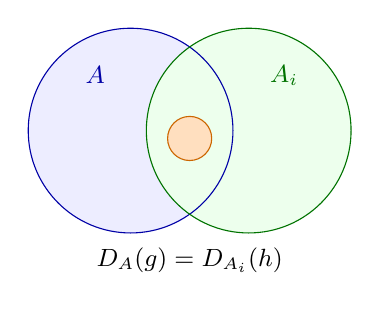
\begin{tikzpicture}[every node/.style={font=\small}]
\fill[blue!7] (-.75,0) circle (1.3);
\fill[green!7] (.75,0) circle (1.3);
\draw[blue!65!black] (-.75,0) circle (1.3);
\draw[green!45!black] (.75,0) circle (1.3);
\node[blue!65!black] at (-1.2,.7) {$\Spec A$};
\node[green!45!black] at (1.2,.7) {$\Spec A_i$};
\filldraw[fill=orange!25,draw=orange!80!black] (0,-.1) circle (.28);
\node at (0,-1.65) {$D_A(g)=D_{A_i}(h)$};
\end{tikzpicture}
\end{center}

\emph{Qué buscamos.} Ver que ser noetheriano pasa a básicos y se comprueba en cubiertas por básicos. \emph{Idea.} Recuperar un ideal como intersección de las contracciones de sus localizaciones y usar cadenas ascendentes.

\begin{prop}[Noetheriano es afín-local]
\label{prop:s09-noetheriano-afin-local}
\begin{enumerate}[label=(\alph*)]
\item Si $A$ es noetheriano, también lo es $A_f$.
\item Si $(f_1,\ldots,f_n)=A$ y cada $A_{f_i}$ es noetheriano, entonces $A$ es noetheriano.
\end{enumerate}
\emph{[Vakil, prop.~5.3.3(a); Atiyah--Macdonald, cap.~7.]}
\end{prop}
\begin{proof}
Para (a), todo ideal de $A_f$ es el extendido de su contracción a $A$. Esta contracción es finitamente generada y sus generadores generan también el ideal localizado.

Para (b), si $\varphi_i:A\to A_{f_i}$ e $I\subseteq A$ es un ideal, afirmamos
\[
I=\bigcap_{i=1}^n\varphi_i^{-1}(IA_{f_i}).
\]
\noindent
\begin{tabular}{@{}p{.51\linewidth}p{.45\linewidth}@{}}
\textbf{Qué hacemos} & \textbf{Por qué se vale}\\[2pt]
\hline
Todo $x\in I$ está en la intersección.
& Su imagen en cada $A_{f_i}$ pertenece a $IA_{f_i}$.\\[4pt]
Si $x$ está en la intersección, para cada $i$ existe $N_i$ con $f_i^{N_i}x\in I$. Tomamos un exponente común $N\ge1$. De $1=\sum_i g_if_i^N$ se sigue que $x=\sum_i g_if_i^Nx\in I$.
& Escribimos $x/1=y_i/f_i^{m_i}$ con $y_i\in I$. Por la \cref{prop:s09-localizacion}, algún $f_i^{r_i}$ anula $f_i^{m_i}x-y_i$, así que sirve $N_i=r_i+m_i$. Las potencias generan $A$ por la \cref{prop:s09-cubrimientos-basicos}.\\[4pt]
Una cadena ascendente de ideales $I_j$ se estabiliza en cada $A_{f_i}$ desde un índice $j_i$. La fórmula de intersección da $I_j=I_J$ para $j\ge J$, con $J=\max_i j_i$.
& Cada $A_{f_i}$ es noetheriano y hay un número finito de localizaciones.
\end{tabular}
\par\smallskip
La fórmula usa contracciones y vale aunque algún mapa $\varphi_i$ tenga núcleo no nulo.
\end{proof}

\emph{Qué buscamos.} Leer lo localmente noetheriano en cualquier abierto afín.

\begin{coro}[Localmente noetheriano en afines]
\label{coro:s09-localmente-noetheriano}
Un esquema $X$ es localmente noetheriano si y solo si $\mathcal O(U)$ es noetheriano para todo abierto afín $U\subseteq X$. Es noetheriano si y solo si además es cuasicompacto. \emph{[Vakil, \S5.3.2--5.3.4; Liu, prop.~3.46(b) y ej.~3.16.]}
\end{coro}
\begin{proof}
La \cref{prop:s09-noetheriano-afin-local} verifica las dos condiciones del \myref{lema:s09-comunicacion-afin} para la propiedad de tener anillo noetheriano. La recíproca y la última afirmación son la definición.
\end{proof}

\emph{Qué buscamos.} Ver que un esquema noetheriano tiene finitas piezas. \emph{Idea.} Pasar de anillos a espacios noetherianos y aplicar inducción noetheriana a los cerrados.

\begin{prop}[Finitud en esquemas noetherianos]
\label{prop:s09-finitud-noetherianos}
Si $X$ es noetheriano:
\begin{enumerate}[label=(\alph*)]
\item su espacio topológico es noetheriano;
\item tiene finitas componentes irreducibles;
\item tiene finitas componentes conexas, cada una unión de componentes irreducibles.
\end{enumerate}
En particular, un anillo noetheriano tiene finitos primos minimales. \emph{[Vakil, ej.~5.1.C, 5.3.B y prop.~3.6.15; Liu, prop.~4.5(c) y 4.9.]}
\end{prop}
\begin{proof}
Si $A$ es noetheriano, una cadena descendente de cerrados $Z_j$ de $\Spec A$ da una cadena ascendente de ideales $I(Z_j)=\bigcap_{\mathfrak p\in Z_j}\mathfrak p$. Esta se estaciona, y $Z_j=V(I(Z_j))$ por la \cref{prop:s09-nilradical}. Una cadena de cerrados en $X$ se estaciona al restringirla a cada miembro de una cubierta afín noetheriana finita. Tomando el máximo de los índices de estabilización obtenemos (a).

En un espacio noetheriano, todo cerrado es unión finita de cerrados irreducibles: de lo contrario elegimos un cerrado minimal que no lo sea. No puede ser irreducible; al escribirlo como unión de dos cerrados propios, la minimalidad da descomposiciones finitas de ambos, contradicción. Aplicado a $X$, sus componentes están entre los finitos irreducibles de una descomposición, y da (b).

Cada componente irreducible es conexa. Agrupamos las que pueden enlazarse mediante una cadena de intersecciones no vacías. Cada grupo tiene unión conexa; su unión es cerrada y su complemento es también cerrado, por ser uniones finitas de componentes. Así esos grupos son las componentes conexas y prueba (c). La correspondencia de la \cref{prop:s09-irreducibles-espectro}(c) da la afirmación sobre primos minimales.
\end{proof}

\begin{ejem}[Noetherianos y no noetherianos]
\label{ejem:s09-noetherianos}
Son noetherianos $\Spec A$ para un DVR $A$, pues es un dominio de ideales principales, y $\Spec\mathbb Z[t]$, por el teorema de la base de Hilbert. Si $A$ es noetheriano, lo son $\mathbb A^n_A$ y $\mathbb P^n_A$: basta una carta en el primer caso y las $n+1$ cartas del segundo tienen anillos de polinomios sobre $A$. En particular, esto vale sobre $k$ y sobre $\mathbb Z$. Un esquema de tipo finito sobre un anillo noetheriano también es noetheriano.
\begin{enumerate}[label=(\alph*)]
\item $\Spec k[x_1,x_2,\ldots]$ no es noetheriano ni localmente noetheriano: su anillo no lo es, por la cadena estricta $(x_1)\subsetneq(x_1,x_2)\subsetneq\cdots$, y aplicamos el \cref{coro:s09-localmente-noetheriano} al afín entero.
\item Si $I$ es infinito, $\coprod_{i\in I}\Spec k$ es localmente noetheriano pero no noetheriano. Sus puntos son abiertos que lo cubren sin subcubierta finita; cada punto es una componente irreducible.
\end{enumerate}
\emph{[Vakil, ej.~3.6.R, 5.1.C, \S5.3.6, ej.~3.6.T, \S3.6.18, ej.~4.3.E(b) y \S3.6.6.]}
\end{ejem}

\begin{obs}
\label{obs:s09-secciones-globales-noetherianas}
El anillo de secciones globales de un esquema noetheriano puede no ser noetheriano. \emph{[Vakil, \S5.3.5.]}
\end{obs}

\begin{ejem}[Los dos ejemplos del programa y tabla resumen]
\label{ejem:s09-tabla-propiedades}
El esquema $\Spec k[\varepsilon]/(\varepsilon^2)$ es noetheriano, irreducible, no reducido y no integral. El esquema $\Spec k[x,y]/(xy)$ es noetheriano, reducido, conexo, no irreducible y no integral; su anillo local en el origen no es dominio. Ambos son noetherianos por ser cocientes de anillos de polinomios.
\begin{center}
\footnotesize
\setlength{\tabcolsep}{4pt}
\renewcommand{\arraystretch}{1.25}
\begin{tabular}{lcccc}
\hline
Esquema & Reducido & Irreducible & Integral & Noetheriano\\
\hline
$\Spec k[\varepsilon]/(\varepsilon^2)$ & no & sí & no & sí\\
$\Spec k[x,y]/(xy)$ & sí & no & no & sí\\
$\Spec(k\times k)$, $\Spec\mathbb Z/6\mathbb Z$ & sí & no & no & sí\\
$\Spec\mathbb Z/4\mathbb Z$ & no & sí & no & sí\\
$\mathbb A^n_A$, $\mathbb P^n_A$, con $A=k,\mathbb Z$ & sí & sí & sí & sí\\
$\Spec\mathbb Z$, $\Spec\mathbb Z[i]$, $\Spec$ de un DVR & sí & sí & sí & sí\\
$\Spec k[x_1,x_2,\ldots]$ & sí & sí & sí & no\\
$\coprod_{\mathbb N}\Spec k$ & sí & no & no & no (localmente sí)\\
\hline
\end{tabular}
\end{center}
\emph{[Vakil, \S3.2.12, ej.~3.7.I y sugerencia del ej.~5.3.C; la tabla es cálculo elemental.]}
\end{ejem}
\begin{proof}
El primer ejemplo se trató en el \cref{ejem:s09-numeros-duales}; su único punto hace irreducible su espectro. Para los ejes, $x,y$ son primos no asociados en $k[x,y]$, y $(xy)=(x)\cap(y)$ por la \cref{prop:s09-polinomios}; esta intersección es radical. Así el cociente es reducido, pero tiene las dos componentes del \cref{ejem:s09-dos-ejes}. En el tallo del origen, $\bar x\bar y=0$ y ninguna clase es nula: si $h\notin(x,y)$ anulara a $\bar x$, tendríamos $hx\in(xy)$ y $y\mid h$, contradiciendo $h\notin(x,y)$; igual para $\bar y$.

Los productos de dos cuerpos tienen dos puntos, son reducidos y noetherianos. En $\mathbb Z/4\mathbb Z$, la clase de $2$ es un nilpotente no nulo y hay un único primo. Los ejemplos sobre $k$, sobre $\mathbb Z$ y sobre un DVR se deducen de los \cref{ejem:s09-reducidos,ejem:s09-integrales,ejem:s09-noetherianos}. El anillo con infinitas variables es dominio, pero no noetheriano; la unión disjunta infinita es reducida, tiene muchas componentes y es solo localmente noetheriana.
\end{proof}

\subsection{Los cocientes de \texorpdfstring{$\mathbb Z[i]$}{Z[i]} por un primo, leídos con los adjetivos}
\emph{Qué buscamos.} Aplicar los cuatro adjetivos a los espectros de los cocientes.

\begin{ejem}[{$\mathbb Z[i]$ y sus cocientes por $p$}]
\label{ejem:s09-adjetivos-fibras}
El anillo $\mathbb Z[t]/(t^2+1)\cong\mathbb Z[i]$ es dominio, de modo que su espectro es integral y noetheriano. Sus cocientes por $p$ se calcularon en el \cref{ejem:s09-enteros-gaussianos}:
\begin{center}
\small
\renewcommand{\arraystretch}{1.25}
\setlength{\tabcolsep}{4pt}
\begin{tabular}{clcccc}
\hline
$p$ & $\mathbb Z[i]/(p)$ & Reducido & Irreducible & Integral & Noetheriano\\
\hline
$2$ & $\mathbb F_2[\varepsilon]/(\varepsilon^2)$ & no & sí & no & sí\\
$3$ & $\mathbb F_9$, un cuerpo & sí & sí & sí & sí\\
$5$ & $\mathbb F_5\times\mathbb F_5$, dos puntos & sí & no & no & sí\\
\hline
\end{tabular}
\end{center}
La primera fila es el \cref{ejem:s09-numeros-duales} con $k=\mathbb F_2$. Un cociente por $p$ de un dominio puede no ser reducido, en $p=2$, ni irreducible, en $p=5$. La \cref{obs:s09-parabola-vakil} presenta el mismo patrón para $y^2=x$. \emph{[Vakil, ej.~10.3.D y ej.~10.3.4.]}
\end{ejem}

\emph{Qué buscamos.} Una familia integral cuya fibra especial sean dos ejes. \emph{Idea.} Reescribir con potencias de $x$ o de $y$ y sustituir $y=\varpi x^{-1}$.

\begin{prop}[La familia $xy=\varpi$]
\label{prop:s09-familia-nodal}
Sea $A$ un DVR con uniformizante $\varpi$, cuerpo de fracciones $K$ y cuerpo residual $\kappa=A/(\varpi)$. Ponemos $R=A[x,y]/(xy-\varpi)$. Entonces $R$ es dominio, $\Spec R$ es integral y noetheriano, y $R/\varpi R\cong\kappa[x,y]/(xy)$, cuyo espectro es reducido, conexo y no integral. \emph{[Liu, \S8.3, ej.~3.53 y \S4.1, lema~1.18; la prueba es un cálculo directo.]}
\end{prop}
\begin{proof}
Usando $xy=\varpi$, todo elemento de $R$ se escribe
\[
c+\sum_{i\ge1}a_ix^i+\sum_{j\ge1}b_jy^j
\]
con sumas finitas y coeficientes en $A$. La sustitución $y=\varpi x^{-1}$ define $R\to K[x,x^{-1}]$ y lleva esta expresión a $c+\sum_i a_ix^i+\sum_j b_j\varpi^jx^{-j}$. Si es cero, la independencia de las potencias de Laurent da $c=a_i=b_j\varpi^j=0$; como $A$ es dominio, todos los $b_j$ son cero. El mapa es inyectivo y $R$ es dominio. Por Hilbert, $R$ es noetheriano, y el \cref{coro:s09-afin-integral} da integralidad. Reducir módulo $\varpi$ da $\kappa[x,y]/(xy)$, y los \cref{ejem:s09-dos-ejes,ejem:s09-tabla-propiedades} dan sus propiedades.
\end{proof}

\begin{samepage}
\section{Ejercicios de reducido, irreducible, integral y noetheriano}

\subsection*{Afirmaciones para completar en casa}

El profesor señaló estas seis afirmaciones para completar en casa. Algunas forman parte de la tarea final del curso.
\begin{itemize}
\item La reducción se lee en las secciones de todo abierto, \cref{prop:s09-reducido-afines}(b).
\item Un cubrimiento por afines reducidos da un esquema reducido, \cref{prop:s09-reducido-afines}(c).
\item El criterio de irreducibilidad de $V(I)$ por el radical de $I$, \cref{prop:s09-irreducibles-espectro}(a).
\item El criterio de irreducibilidad de $\Spec A$ por el nilradical y los primos minimales, \cref{prop:s09-irreducibles-espectro}(d).
\item Todo esquema integral es reducido e irreducible, \cref{prop:s09-integral-equivalencia}.
\item El dominio $A[x,y]/(xy-\varpi)$ y su cociente módulo $\varpi$, \cref{prop:s09-familia-nodal}.
\end{itemize}
\end{samepage}

\begin{ejer}
\label{ejer:s09-clasificar-anillos}
Decide si $\Spec A$ es reducido, irreducible, integral y noetheriano para cada anillo, con $k$ un cuerpo:
\begin{enumerate}[label=(\alph*)]
\item $A=\mathbb Z/12\mathbb Z$.
\item $A=k[x,y]/(x^2-y^2)$ con $\operatorname{car}k\ne2$.
\item $A=k[x,y]/(x^2-y^3)$.
\item $A=\mathbb Z[x]/(x^2+1)$ y $A=\mathbb Z[x]/(x^2-1)$.
\item $A=k[x]/(x^2(x-1))$.
\end{enumerate}
\emph{[Liu, ej.~4.1; Vakil, ej.~3.7.H.]}
\end{ejer}

\begin{ejer}
\label{ejer:s09-componentes-plano-recta}
Sea $k$ un cuerpo. Calcula las componentes irreducibles de $\Spec k[x,y,z]/(xz,yz)$, di cuáles son sus primos minimales y decide si es reducido. Dibuja el espacio e indica dónde se cortan sus componentes. \emph{[Vakil, ej.~3.7.I; Liu, ej.~4.8.]}
\end{ejer}

\begin{ejer}
\label{ejer:s09-irreducible-no-afin-local}
Muestra que ser irreducible no cumple la condición (ii) del \myref{lema:s09-comunicacion-afin}. \emph{Pista.} Con $A=k\times k$, sean $f_1=(1,0)$ y $f_2=(0,1)$. \emph{[Vakil, \S5.3.2 y ej.~3.6.A.]}
\end{ejer}

\begin{ejer}
\label{ejer:s09-espacio-noetheriano-esquema-no}
Sea $k$ un cuerpo y $A=k[x_1,x_2,\ldots]/(x_ix_j:i,j\ge1)$. Muestra que $\Spec A$ es un espacio noetheriano y no es un esquema noetheriano. \emph{Pista.} Describe sus primos y usa el \cref{coro:s09-localmente-noetheriano}. \emph{[Vakil, observación final del ej.~3.6.T.]}
\end{ejer}

\begin{ejer}
\label{ejer:s09-cuadratico-integral}
Sea $n\in\mathbb Z$. Demuestra que $\Spec\mathbb Z[t]/(t^2-n)$ es integral si y solo si $n$ no es un cuadrado en $\mathbb Z$. \emph{[Vakil, ej.~5.2.H.]}
\end{ejer}

\begin{ejer}
\label{ejer:s09-adjetivos-raiz-dos}
Para $p=2,3,7$, describe con los cuatro adjetivos el esquema $\Spec\mathbb F_p[t]/(t^2-2)$, que es la fibra de $\Spec\mathbb Z[t]/(t^2-2)\to\Spec\mathbb Z$ sobre $(p)$. \emph{Pista.} Factoriza $t^2-2$ módulo cada primo, como en el \cref{ejem:s09-enteros-gaussianos}. \emph{[Vakil, ej.~10.3.D.]}
\end{ejer}

\section{Ejercicios de valoración discreta, reducción y \texorpdfstring{$\mathbb P^n_A$}{PnA}}

\begin{ejer}[Valuaciones]
\label{ejer:s09-valuaciones}
Calcula $v_p(30/49)$ para $p=2,3,5,7$. Describe el anillo de valuación de $v(f)=-\deg f$ en $k(x)$, el ejemplo (iii) de Vakil, \S13.5.5, como un conjunto de fracciones y muestra que es $k[u]_{(u)}$ con $u=1/x$. \emph{[Vakil, ej.~13.5.B.]}
\end{ejer}

\begin{ejer}[Reducción de puntos]
\label{ejer:s09-reduccion-puntos}
Reduce $t=5/7$, $t=7/9$ y $t=11/6$ de $\mathbb P^1(\mathbb Q)$ módulo $p=2,3,5,7$, escribiendo cada punto como $[a:b]$ con $a,b$ enteros primos entre sí y $t=b/a$, según la \cref{defi:s09-recta-proyectiva}.
\end{ejer}

\begin{ejer}[Modelos étale de $t^2-n$]
\label{ejer:s09-modelos-etale}
Determina los primos $p$ para los que el morfismo
\[
\Spec\mathbb Z_{(p)}[t]/(t^2-n)\longrightarrow\Spec\mathbb Z_{(p)}
\]
es étale en los puntos de la fibra especial, para $n=2,3,5,6$.
\end{ejer}

\begin{ejer}[Los primos de $\mathbb Z\lbrack t\rbrack/(t^2-n)$ sobre cada primo]
\label{ejer:s09-primos-cuadraticos-reduccion}
Sea $n\in\set{2,3,5,6}$. Para cada primo $p\le11$, decide cuántos primos de $\mathbb Z[t]/(t^2-n)$ están sobre $(p)$, es decir, cuántos primos tiene $\mathbb F_p[t]/(t^2-n)$, y si ese anillo tiene un nilpotente no nulo. Concluye para qué primos $p$ hay un nilpotente no nulo. \emph{[Cálculo elemental, como en el \cref{ejem:s09-enteros-gaussianos}; Vakil, ej.~10.3.D.]}
\end{ejer}

\begin{ejer}[Tres puntos y sus reducciones]
\label{ejer:s09-tres-puntos}
Sea $n\ge1$ entero. Para cada primo $p$, determina cuáles de $t=0$, $t=n$ y $t=n^2$ en $\mathbb P^1(\mathbb Q)$ tienen la misma reducción módulo $p$. Describe el resultado para $n=6$.
\end{ejer}

\begin{ejer}[Pegados inversos en $\mathbb P^2_A$]
\label{ejer:s09-pegados-inversos}
Con las fórmulas del \cref{ejem:s09-pegados-plano-proyectivo}, calcula $\varphi_{10}$ y $\varphi_{21}$ y comprueba que $\varphi_{10}\circ\varphi_{01}$ es la identidad de $D(u)\subseteq U_0$ y $\varphi_{21}\circ\varphi_{12}$ es la identidad de $D(v')\subseteq U_1$. Describe el complemento de $U_0$ en $\mathbb P^2_A$.
\end{ejer}

La próxima clase tratará morfismos de esquemas y subesquemas. El profesor anunció la correspondencia $\operatorname{Hom}(X,\Spec A)\cong\operatorname{Hom}(A,\Gamma(X,\mathcal O_X))$.
